\SourceLeaf{281}%
\noindent wo $\varepsilon$ entweder $+1$ oder $-1$ und das Zeichen von $x$
unbestimmt bleibt; doch, weil nemlich zum Compagnon von $n$, $m$ gehört:

\[
\begin{array}{ccc}
y&&x \\
&m& \\
&-\varepsilon.&
\end{array}
\]

\noindent Hiernach werden in Folge des Paradigma die Grössen $(a), (b),
(c)$ etc.\ leicht bestimmt.

Bezeichnet man nun den Character irgend eines Flächentheils, der
z.\,B. an die $+$ oder $-$Seite von $a$ grenzt, durch $\mathrm{Ch}\pm a$
und die Werthe von $(a), (b)$ etc.\ für $a=b=c=d=e=\text{etc.}=1$, durch
$A:a$, so ist

\[
2\,\mathrm{Ch}\,\varepsilon a - \varepsilon - A:a = \text{Const.} = k,
\]

\noindent und ist die Area der Figur $= \Omega$, so ist die ganze Seitenabweichung
nach der $+$Seite

\[
= k\,.\,360^0 - \frac{\Omega\,.\,720^0}{\text{Fläche der Kugel}}.
\]

\Needspace{5\baselineskip}\begin{center}[5.]\end{center}

\begin{center}\resizebox{11.0cm}{!}{%
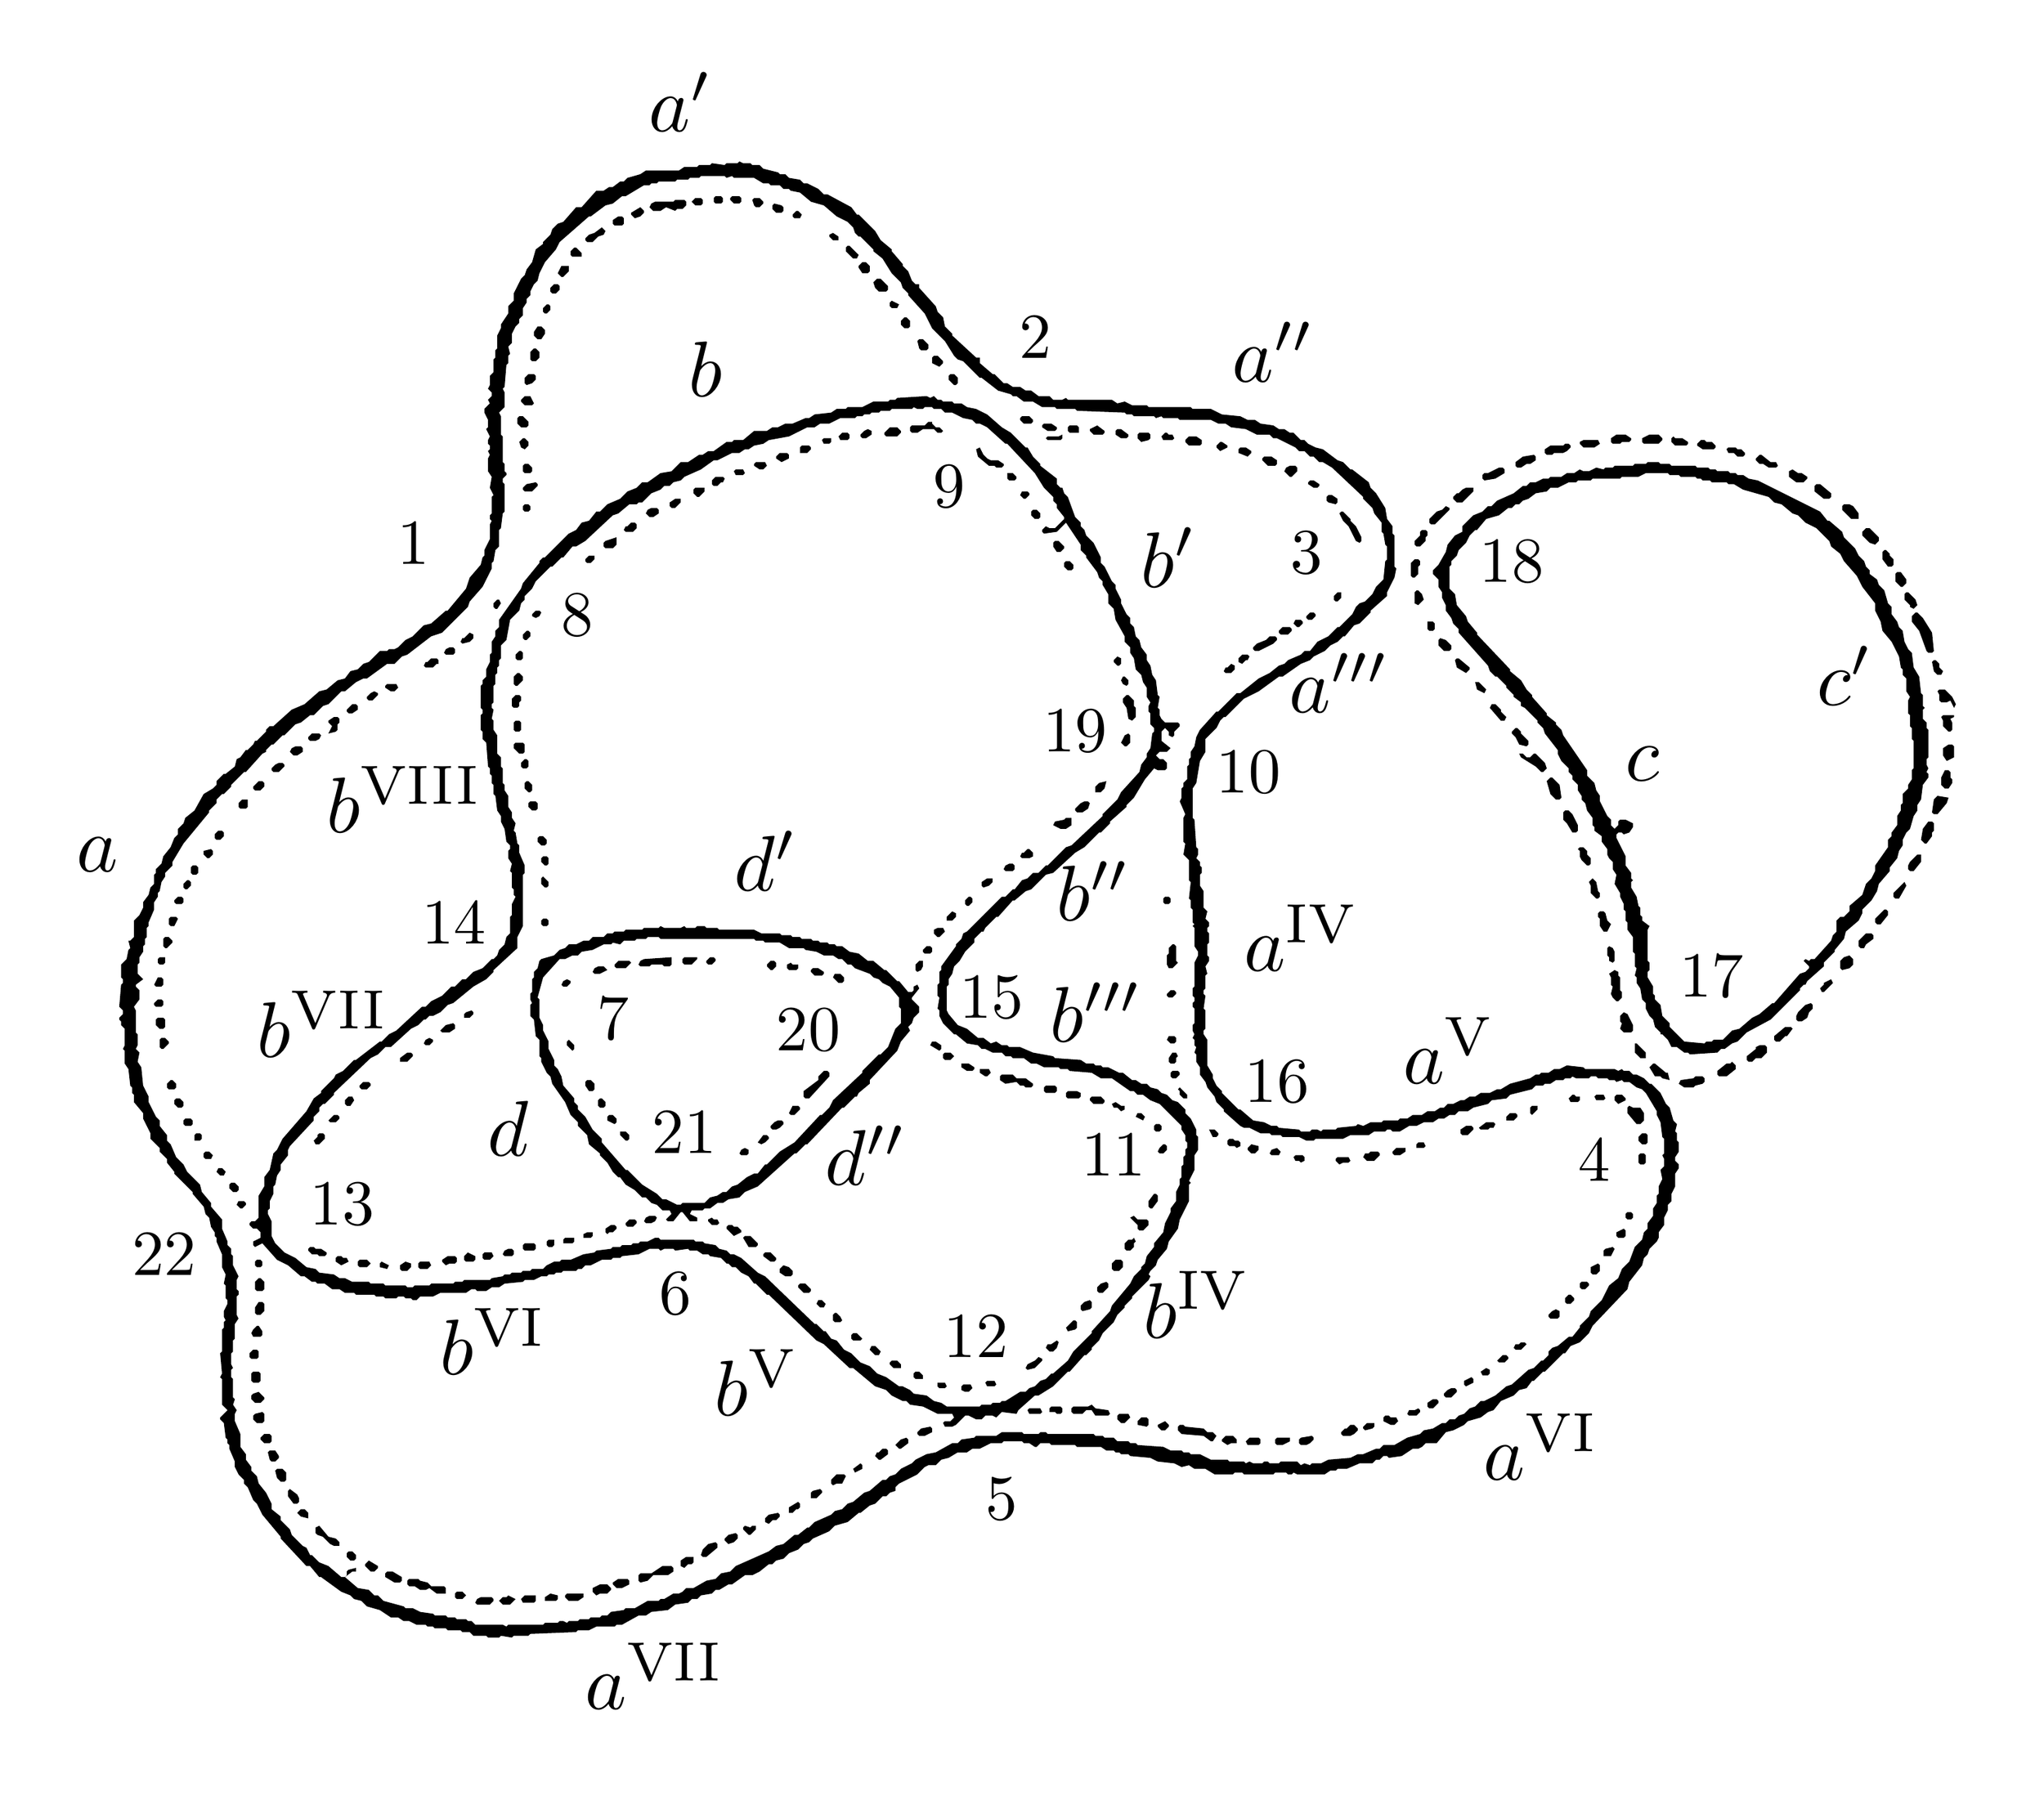
\begin{tikzpicture}[x=1pt,y=-1pt]
\path[use as bounding box] (0,0) rectangle (1094,964);
\path[fill=black,draw=none,even odd rule]
(919,578) -- (918,577) -- (914,577) -- (913,578) -- (906,579) -- (905,581) -- (908,583) -- (913,583) -- (914,582) -- (918,581) -- (919,580) -- cycle
(889,572) -- (892,577) -- (895,577) -- (896,578) -- (900,579) -- (899,575) -- (898,575) -- (892,570) -- (891,570) -- cycle
(936,571) -- (934,569) -- (933,570) -- (931,570) -- (926,574) -- (926,576) -- (927,577) -- (931,577) -- (936,573) -- cycle
(953,561) -- (952,560) -- (949,560) -- (947,561) -- (947,562) -- (942,566) -- (942,568) -- (943,569) -- (945,569) -- (947,567) -- (950,567) -- (953,564) -- cycle
(881,559) -- (881,564) -- (884,567) -- (887,567) -- (887,564) -- (882,559) -- cycle
(967,551) -- (966,550) -- (963,550) -- (957,555) -- (957,557) -- (958,558) -- (960,558) -- (963,555) -- (964,555) -- cycle
(875,542) -- (873,544) -- (873,547) -- (874,548) -- (873,551) -- (875,553) -- (879,553) -- (880,552) -- (880,549) -- (877,543) -- cycle
(977,537) -- (974,538) -- (970,542) -- (969,544) -- (969,546) -- (970,547) -- (972,547) -- (975,545) -- (976,542) -- (978,540) -- (978,538) -- cycle
(988,524) -- (984,526) -- (984,527) -- (982,529) -- (983,531) -- (984,531) -- (989,526) -- cycle
(870,519) -- (867,521) -- (868,523) -- (868,527) -- (869,528) -- (868,532) -- (869,534) -- (871,536) -- (872,536) -- (874,534) -- (874,531) -- (873,530) -- (873,523) -- (872,522) -- (872,520) -- cycle
(998,511) -- (995,512) -- (993,514) -- (993,518) -- (994,519) -- (998,518) -- (1000,516) -- (1000,513) -- cycle
(867,506) -- (866,507) -- (866,511) -- (867,512) -- (867,514) -- (869,515) -- (870,514) -- (870,509) -- (869,507) -- cycle
(1010,499) -- (1007,499) -- (1003,503) -- (1003,506) -- (1004,507) -- (1006,507) -- (1007,505) -- (1011,502) -- (1011,500) -- cycle
(862,487) -- (861,488) -- (861,490) -- (862,491) -- (862,495) -- (864,498) -- (866,498) -- (868,494) -- (866,492) -- (865,488) -- (864,487) -- cycle
(1018,486) -- (1017,486) -- (1012,491) -- (1012,493) -- (1013,494) -- (1015,494) -- (1019,489) -- (1019,487) -- cycle
(1028,471) -- (1022,477) -- (1022,479) -- (1023,480) -- (1025,480) -- (1029,473) -- cycle
(858,469) -- (856,471) -- (857,473) -- (857,477) -- (860,480) -- (861,480) -- (862,479) -- (862,477) -- (861,476) -- (860,471) -- cycle
(1037,456) -- (1035,456) -- (1031,460) -- (1030,462) -- (1030,464) -- (1031,465) -- (1033,465) -- (1037,460) -- cycle
(851,452) -- (850,453) -- (851,454) -- (851,457) -- (852,459) -- (855,462) -- (856,462) -- (857,461) -- (857,458) -- (855,456) -- (855,454) -- (853,452) -- cycle
(1043,438) -- (1041,438) -- (1038,442) -- (1037,448) -- (1039,450) -- (1040,450) -- (1043,446) -- (1043,444) -- (1044,443) -- (1044,439) -- cycle
(843,432) -- (842,433) -- (842,437) -- (844,439) -- (847,444) -- (849,444) -- (850,443) -- (850,440) -- (847,434) -- (845,432) -- cycle
(1052,425) -- (1046,424) -- (1044,426) -- (1043,433) -- (1044,434) -- (1046,434) -- (1051,428) -- cycle
(835,414) -- (833,416) -- (835,423) -- (838,426) -- (840,426) -- (841,425) -- (840,418) -- (836,414) -- cycle
(1050,410) -- (1048,414) -- (1048,418) -- (1050,420) -- (1052,420) -- (1054,417) -- (1054,415) -- (1053,414) -- (1053,411) -- (1052,410) -- cycle
(818,401) -- (819,403) -- (827,408) -- (830,411) -- (831,411) -- (833,409) -- (832,406) -- (827,401) -- (826,401) -- (824,403) -- (822,403) -- (820,401) -- cycle
(1054,396) -- (1052,396) -- (1049,398) -- (1049,402) -- (1051,405) -- (1055,403) -- (1055,397) -- cycle
(816,387) -- (814,389) -- (814,390) -- (816,392) -- (818,396) -- (822,397) -- (823,396) -- (823,394) -- (819,390) -- (819,389) -- (817,387) -- cycle
(1049,380) -- (1048,381) -- (1049,383) -- (1049,386) -- (1052,389) -- (1053,389) -- (1054,388) -- (1054,384) -- (1053,382) -- (1055,381) -- (1055,380) -- cycle
(803,374) -- (802,376) -- (808,383) -- (810,383) -- (811,381) -- (808,378) -- (808,377) -- (805,374) -- cycle
(1047,366) -- (1046,367) -- (1047,369) -- (1047,372) -- (1048,373) -- (1051,373) -- (1053,372) -- (1055,376) -- (1056,374) -- (1054,370) -- (1050,366) -- cycle
(794,362) -- (795,366) -- (799,368) -- (800,366) -- (796,362) -- cycle
(1044,350) -- (1043,351) -- (1044,356) -- (1046,358) -- (1048,358) -- (1049,356) -- (1047,354) -- (1047,352) -- (1045,350) -- cycle
(784,349) -- (783,350) -- (784,354) -- (789,357) -- (791,355) -- (791,354) -- (785,349) -- cycle
(775,338) -- (774,339) -- (774,342) -- (777,345) -- (780,345) -- (781,344) -- (781,342) -- (778,339) -- cycle
(768,329) -- (768,333) -- (769,334) -- (771,334) -- (772,333) -- (772,330) -- (771,329) -- cycle
(1034,324) -- (1032,326) -- (1032,329) -- (1036,334) -- (1040,345) -- (1041,346) -- (1043,346) -- (1044,345) -- (1043,335) -- (1038,327) -- (1035,324) -- cycle
(1029,313) -- (1028,314) -- (1028,317) -- (1031,320) -- (1031,321) -- (1033,322) -- (1035,320) -- (1034,317) -- (1030,313) -- cycle
(762,312) -- (761,313) -- (761,319) -- (763,320) -- (766,317) -- (765,314) -- (763,312) -- cycle
(1024,302) -- (1023,303) -- (1023,307) -- (1026,310) -- (1027,310) -- (1029,308) -- (1029,306) -- (1026,302) -- cycle
(763,295) -- (761,295) -- (759,297) -- (759,304) -- (760,305) -- (761,305) -- (763,303) -- (763,299) -- (764,298) -- (764,296) -- cycle
(1017,290) -- (1016,291) -- (1016,295) -- (1019,299) -- (1021,299) -- (1022,298) -- (1022,295) -- (1020,293) -- (1020,292) -- (1018,290) -- cycle
(767,279) -- (765,279) -- (764,280) -- (764,282) -- (761,285) -- (761,287) -- (762,288) -- (764,288) -- (767,285) -- (767,283) -- (768,282) -- (768,280) -- cycle
(1007,278) -- (1005,280) -- (1005,282) -- (1009,286) -- (1012,287) -- (1014,285) -- (1014,283) -- (1009,278) -- cycle
(780,267) -- (778,266) -- (776,268) -- (773,269) -- (769,273) -- (769,275) -- (770,276) -- (772,276) -- (780,268) -- cycle
(994,266) -- (994,268) -- (999,273) -- (1003,273) -- (1003,270) -- (1000,266) -- (998,265) -- (995,265) -- cycle
(793,256) -- (789,256) -- (787,257) -- (785,259) -- (784,259) -- (782,261) -- (782,262) -- (784,264) -- (787,264) -- (793,258) -- cycle
(980,254) -- (979,255) -- (979,258) -- (984,262) -- (987,262) -- (988,261) -- (988,259) -- (982,254) -- cycle
(965,247) -- (965,250) -- (969,253) -- (973,253) -- (975,251) -- (975,250) -- (972,248) -- (970,248) -- (967,246) -- cycle
(810,246) -- (809,245) -- (807,245) -- (801,248) -- (799,248) -- (798,249) -- (798,251) -- (799,252) -- (805,251) -- (810,248) -- cycle
(851,246) -- (848,248) -- (844,248) -- (841,250) -- (835,250) -- (834,251) -- (831,251) -- (827,253) -- (824,253) -- (822,255) -- (820,255) -- (815,259) -- (806,263) -- (803,266) -- (801,266) -- (798,269) -- (793,271) -- (787,277) -- (787,280) -- (783,282) -- (779,287) -- (778,291) -- (774,298) -- (771,301) -- (771,303) -- (774,306) -- (774,310) -- (776,313) -- (776,316) -- (778,320) -- (778,323) -- (781,327) -- (782,330) -- (785,333) -- (785,335) -- (801,353) -- (802,356) -- (805,359) -- (806,359) -- (811,364) -- (811,365) -- (815,369) -- (815,370) -- (819,373) -- (819,375) -- (821,376) -- (828,383) -- (828,384) -- (831,387) -- (832,390) -- (839,399) -- (839,401) -- (841,405) -- (845,409) -- (845,411) -- (847,413) -- (847,415) -- (850,418) -- (850,421) -- (852,424) -- (852,426) -- (854,428) -- (855,432) -- (858,436) -- (858,440) -- (859,441) -- (859,443) -- (863,446) -- (863,449) -- (866,453) -- (866,456) -- (867,458) -- (869,460) -- (869,464) -- (871,467) -- (870,472) -- (873,477) -- (873,479) -- (875,483) -- (875,486) -- (876,487) -- (876,492) -- (877,493) -- (877,497) -- (880,501) -- (880,509) -- (881,510) -- (881,517) -- (882,518) -- (881,522) -- (882,523) -- (882,526) -- (884,529) -- (885,535) -- (887,537) -- (887,540) -- (889,544) -- (891,546) -- (892,550) -- (895,553) -- (895,554) -- (896,554) -- (899,557) -- (901,561) -- (904,561) -- (908,564) -- (910,564) -- (911,565) -- (926,564) -- (928,562) -- (930,562) -- (934,559) -- (937,558) -- (942,553) -- (955,546) -- (971,530) -- (971,529) -- (973,527) -- (974,527) -- (975,525) -- (984,517) -- (984,515) -- (990,509) -- (990,508) -- (995,502) -- (996,498) -- (1003,492) -- (1005,488) -- (1005,486) -- (1010,481) -- (1013,476) -- (1014,472) -- (1020,465) -- (1020,463) -- (1024,458) -- (1025,454) -- (1027,451) -- (1027,448) -- (1029,444) -- (1031,442) -- (1033,435) -- (1035,432) -- (1035,429) -- (1037,426) -- (1038,418) -- (1041,414) -- (1041,412) -- (1040,411) -- (1041,409) -- (1040,407) -- (1040,404) -- (1041,403) -- (1041,388) -- (1040,387) -- (1040,384) -- (1038,382) -- (1038,377) -- (1039,376) -- (1038,375) -- (1038,369) -- (1037,368) -- (1036,359) -- (1033,354) -- (1032,346) -- (1030,344) -- (1028,340) -- (1027,334) -- (1025,332) -- (1024,329) -- (1021,325) -- (1021,321) -- (1019,319) -- (1017,312) -- (1014,309) -- (1013,306) -- (1009,303) -- (1009,301) -- (1007,299) -- (1006,296) -- (1003,293) -- (1001,289) -- (995,283) -- (994,280) -- (987,274) -- (986,274) -- (982,269) -- (948,252) -- (943,251) -- (940,249) -- (937,249) -- (936,248) -- (933,248) -- (932,247) -- (926,247) -- (925,246) -- (922,246) -- (921,245) -- (915,245) -- (914,244) -- (901,244) -- (900,243) -- (895,243) -- (894,242) -- (888,242) -- (887,243) -- (881,243) -- (880,244) -- (870,244) -- (869,245) -- (865,245) -- (864,246) -- (860,245) -- (856,247) -- (853,247) -- cycle
(845,253) -- (849,253) -- (850,252) -- (857,252) -- (858,251) -- (873,251) -- (874,250) -- (883,250) -- (887,248) -- (899,248) -- (900,249) -- (905,249) -- (906,250) -- (914,250) -- (915,251) -- (917,251) -- (918,252) -- (922,252) -- (923,253) -- (931,253) -- (932,254) -- (935,254) -- (940,257) -- (954,261) -- (957,264) -- (961,265) -- (967,270) -- (970,271) -- (974,275) -- (980,278) -- (987,285) -- (988,288) -- (993,292) -- (995,296) -- (1002,304) -- (1005,310) -- (1012,319) -- (1012,323) -- (1015,329) -- (1016,334) -- (1021,340) -- (1025,348) -- (1026,354) -- (1027,355) -- (1027,358) -- (1029,360) -- (1029,367) -- (1031,370) -- (1030,372) -- (1030,379) -- (1031,380) -- (1031,386) -- (1032,387) -- (1032,393) -- (1033,394) -- (1033,409) -- (1032,410) -- (1032,415) -- (1030,418) -- (1030,420) -- (1027,423) -- (1027,428) -- (1026,429) -- (1026,432) -- (1024,435) -- (1024,440) -- (1021,444) -- (1021,446) -- (1019,448) -- (1019,452) -- (1012,462) -- (1012,465) -- (1010,469) -- (1007,472) -- (1005,478) -- (998,484) -- (998,487) -- (995,490) -- (993,490) -- (991,492) -- (991,498) -- (989,500) -- (988,503) -- (979,513) -- (977,513) -- (976,514) -- (974,513) -- (973,514) -- (976,517) -- (976,518) -- (974,520) -- (971,521) -- (957,537) -- (956,537) -- (949,543) -- (945,545) -- (938,551) -- (934,552) -- (929,557) -- (924,557) -- (923,558) -- (920,558) -- (919,559) -- (908,558) -- (900,550) -- (900,548) -- (896,544) -- (895,538) -- (892,535) -- (892,533) -- (891,532) -- (891,528) -- (888,523) -- (888,520) -- (889,519) -- (889,515) -- (888,514) -- (888,497) -- (889,495) -- (885,492) -- (885,490) -- (884,489) -- (884,485) -- (883,484) -- (882,479) -- (879,474) -- (879,471) -- (880,470) -- (879,469) -- (879,466) -- (876,462) -- (876,457) -- (871,447) -- (871,445) -- (872,444) -- (874,444) -- (875,445) -- (878,444) -- (880,441) -- (880,439) -- (876,437) -- (873,437) -- (872,438) -- (872,440) -- (870,442) -- (868,440) -- (868,437) -- (866,435) -- (862,427) -- (862,424) -- (860,421) -- (859,417) -- (855,413) -- (855,410) -- (842,391) -- (841,388) -- (838,385) -- (838,384) -- (833,380) -- (833,379) -- (825,370) -- (825,369) -- (822,366) -- (819,361) -- (813,356) -- (813,355) -- (795,336) -- (795,335) -- (790,329) -- (789,326) -- (784,320) -- (783,314) -- (780,311) -- (780,299) -- (781,298) -- (781,296) -- (784,293) -- (785,290) -- (789,286) -- (791,282) -- (794,279) -- (795,279) -- (800,273) -- (807,271) -- (812,267) -- (814,267) -- (816,265) -- (818,265) -- (820,263) -- (823,262) -- (827,259) -- (833,258) -- (835,256) -- (839,256) -- cycle
(947,240) -- (947,241) -- (949,243) -- (951,243) -- (954,245) -- (958,245) -- (959,244) -- (958,242) -- (955,242) -- (950,238) -- (949,238) -- cycle
(827,239) -- (826,238) -- (820,239) -- (816,242) -- (816,244) -- (817,245) -- (819,245) -- (822,243) -- (824,243) -- (827,241) -- cycle
(931,235) -- (932,237) -- (935,237) -- (937,239) -- (940,239) -- (941,238) -- (941,237) -- (939,235) -- (937,235) -- (936,234) -- (932,234) -- cycle
(846,233) -- (845,232) -- (843,232) -- (842,233) -- (835,233) -- (832,235) -- (832,237) -- (833,238) -- (836,238) -- (837,237) -- (842,237) -- (844,236) -- (846,234) -- cycle
(915,232) -- (915,233) -- (918,235) -- (924,235) -- (925,234) -- (925,233) -- (923,231) -- (920,231) -- (919,230) -- (917,230) -- cycle
(851,231) -- (851,232) -- (853,234) -- (859,234) -- (862,232) -- (861,230) -- (853,230) -- cycle
(901,229) -- (901,231) -- (903,233) -- (909,233) -- (910,232) -- (910,231) -- (907,229) -- (903,229) -- (902,228) -- cycle
(885,229) -- (885,231) -- (886,232) -- (894,232) -- (896,230) -- (896,229) -- (894,227) -- (889,227) -- cycle
(868,229) -- (868,231) -- (869,232) -- (873,232) -- (874,231) -- (878,231) -- (879,230) -- (879,229) -- (876,227) -- (871,227) -- cycle
(404,80) -- (400,80) -- (399,79) -- (395,79) -- (393,78) -- (392,79) -- (386,79) -- (385,80) -- (378,79) -- (377,80) -- (371,80) -- (370,81) -- (363,81) -- (360,83) -- (342,83) -- (339,85) -- (332,87) -- (330,89) -- (328,89) -- (324,92) -- (322,92) -- (319,94) -- (315,94) -- (307,103) -- (304,103) -- (297,111) -- (294,112) -- (291,115) -- (290,118) -- (286,122) -- (286,123) -- (282,126) -- (280,133) -- (277,137) -- (276,140) -- (274,142) -- (270,150) -- (270,154) -- (267,157) -- (267,161) -- (263,167) -- (263,169) -- (261,173) -- (261,180) -- (260,181) -- (260,185) -- (259,186) -- (259,193) -- (257,195) -- (257,200) -- (256,202) -- (258,204) -- (258,206) -- (256,208) -- (257,210) -- (254,213) -- (254,215) -- (256,219) -- (256,223) -- (255,224) -- (257,228) -- (256,230) -- (256,232) -- (257,233) -- (257,235) -- (256,236) -- (257,238) -- (256,240) -- (256,247) -- (258,250) -- (257,256) -- (259,260) -- (258,261) -- (258,270) -- (257,271) -- (257,273) -- (258,274) -- (257,276) -- (257,284) -- (254,290) -- (254,293) -- (253,294) -- (252,298) -- (246,305) -- (244,311) -- (234,323) -- (233,323) -- (225,330) -- (221,331) -- (215,337) -- (211,339) -- (207,343) -- (205,344) -- (202,344) -- (201,345) -- (197,345) -- (191,351) -- (188,352) -- (185,355) -- (181,356) -- (178,360) -- (174,361) -- (168,366) -- (164,367) -- (156,374) -- (149,377) -- (139,386) -- (137,386) -- (135,388) -- (135,389) -- (130,394) -- (129,394) -- (128,396) -- (125,399) -- (124,399) -- (121,403) -- (119,404) -- (118,408) -- (113,412) -- (112,412) -- (108,416) -- (108,418) -- (106,420) -- (101,423) -- (96,432) -- (91,436) -- (90,439) -- (87,442) -- (87,445) -- (85,447) -- (83,452) -- (79,457) -- (78,461) -- (75,464) -- (75,466) -- (74,467) -- (74,472) -- (72,474) -- (71,478) -- (68,482) -- (68,485) -- (66,489) -- (63,492) -- (63,501) -- (61,503) -- (60,503) -- (61,507) -- (60,508) -- (59,513) -- (56,516) -- (56,523) -- (57,524) -- (57,526) -- (56,527) -- (55,539) -- (57,541) -- (57,543) -- (55,545) -- (55,546) -- (56,547) -- (56,549) -- (58,551) -- (58,560) -- (57,562) -- (58,563) -- (58,570) -- (60,573) -- (61,582) -- (62,583) -- (62,586) -- (63,587) -- (63,591) -- (68,597) -- (68,600) -- (72,608) -- (72,611) -- (77,616) -- (77,618) -- (81,622) -- (81,624) -- (85,629) -- (85,630) -- (95,640) -- (95,641) -- (101,648) -- (102,652) -- (104,654) -- (105,659) -- (107,662) -- (107,664) -- (108,665) -- (108,667) -- (111,674) -- (111,681) -- (113,685) -- (112,690) -- (113,691) -- (113,698) -- (114,699) -- (114,701) -- (112,705) -- (112,708) -- (113,710) -- (112,711) -- (112,714) -- (111,715) -- (111,727) -- (110,728) -- (111,739) -- (110,741) -- (111,742) -- (111,756) -- (114,759) -- (110,763) -- (110,764) -- (112,766) -- (113,774) -- (114,775) -- (114,777) -- (115,778) -- (115,780) -- (118,787) -- (118,790) -- (120,794) -- (123,797) -- (123,799) -- (125,801) -- (128,808) -- (130,810) -- (133,816) -- (143,828) -- (143,829) -- (157,844) -- (159,844) -- (164,850) -- (165,850) -- (176,858) -- (181,860) -- (183,862) -- (187,863) -- (190,866) -- (197,868) -- (203,872) -- (207,872) -- (210,874) -- (213,874) -- (217,876) -- (222,876) -- (223,877) -- (226,877) -- (227,878) -- (233,878) -- (234,879) -- (241,879) -- (242,880) -- (246,880) -- (248,882) -- (255,882) -- (256,883) -- (262,883) -- (263,882) -- (269,883) -- (270,882) -- (278,882) -- (279,881) -- (304,880) -- (305,879) -- (311,879) -- (315,877) -- (325,877) -- (326,876) -- (329,876) -- (338,871) -- (342,871) -- (345,869) -- (354,868) -- (358,865) -- (365,864) -- (367,862) -- (370,862) -- (372,860) -- (378,859) -- (380,857) -- (382,857) -- (387,854) -- (389,854) -- (396,849) -- (400,849) -- (404,847) -- (409,843) -- (411,843) -- (413,841) -- (417,840) -- (420,837) -- (425,835) -- (428,832) -- (431,831) -- (433,829) -- (442,825) -- (445,822) -- (452,820) -- (458,815) -- (459,815) -- (464,811) -- (467,810) -- (471,806) -- (473,806) -- (475,804) -- (478,803) -- (478,801) -- (480,799) -- (490,794) -- (494,790) -- (496,789) -- (500,789) -- (503,786) -- (507,785) -- (512,782) -- (517,782) -- (520,780) -- (524,780) -- (530,777) -- (536,777) -- (537,776) -- (547,776) -- (548,777) -- (551,777) -- (554,779) -- (555,779) -- (557,777) -- (562,777) -- (563,778) -- (576,778) -- (577,779) -- (590,779) -- (593,781) -- (597,781) -- (598,782) -- (600,782) -- (601,783) -- (605,783) -- (606,784) -- (617,785) -- (621,787) -- (630,788) -- (634,790) -- (638,789) -- (641,791) -- (647,791) -- (652,794) -- (662,794) -- (663,793) -- (667,793) -- (668,794) -- (684,794) -- (685,793) -- (691,793) -- (692,794) -- (694,794) -- (695,793) -- (697,794) -- (712,794) -- (715,792) -- (718,792) -- (719,791) -- (724,791) -- (731,788) -- (738,788) -- (740,786) -- (742,786) -- (744,784) -- (746,784) -- (747,785) -- (754,784) -- (760,780) -- (763,780) -- (765,779) -- (767,777) -- (773,777) -- (778,771) -- (782,770) -- (788,767) -- (790,765) -- (797,763) -- (801,760) -- (804,759) -- (808,754) -- (815,751) -- (818,748) -- (822,747) -- (825,743) -- (826,743) -- (831,738) -- (832,738) -- (842,728) -- (843,728) -- (846,724) -- (851,722) -- (856,717) -- (858,713) -- (877,693) -- (878,689) -- (885,680) -- (886,676) -- (888,674) -- (889,671) -- (893,667) -- (894,665) -- (894,662) -- (897,658) -- (897,654) -- (899,650) -- (899,647) -- (901,645) -- (901,641) -- (903,637) -- (903,630) -- (905,627) -- (905,625) -- (903,623) -- (903,621) -- (905,618) -- (905,613) -- (904,612) -- (904,608) -- (903,607) -- (904,603) -- (902,601) -- (900,594) -- (898,592) -- (895,586) -- (890,581) -- (889,581) -- (886,578) -- (882,576) -- (880,576) -- (878,574) -- (875,574) -- (874,573) -- (872,574) -- (870,573) -- (854,573) -- (853,572) -- (844,571) -- (840,573) -- (837,573) -- (834,575) -- (830,575) -- (829,576) -- (827,576) -- (824,578) -- (813,581) -- (808,584) -- (806,584) -- (802,586) -- (797,586) -- (794,588) -- (791,588) -- (788,590) -- (786,590) -- (782,592) -- (779,592) -- (777,594) -- (775,594) -- (772,596) -- (768,596) -- (765,598) -- (760,598) -- (757,600) -- (753,600) -- (752,601) -- (744,601) -- (743,602) -- (737,602) -- (733,604) -- (730,603) -- (729,604) -- (719,605) -- (718,606) -- (711,606) -- (710,607) -- (708,606) -- (705,606) -- (704,607) -- (699,607) -- (698,606) -- (687,605) -- (686,604) -- (683,604) -- (679,602) -- (673,601) -- (666,595) -- (665,595) -- (656,586) -- (656,585) -- (653,582) -- (651,578) -- (651,576) -- (648,571) -- (648,557) -- (646,554) -- (646,552) -- (647,551) -- (647,541) -- (646,540) -- (647,533) -- (646,532) -- (646,530) -- (647,529) -- (647,522) -- (648,521) -- (647,517) -- (649,514) -- (649,512) -- (648,511) -- (648,505) -- (649,504) -- (649,499) -- (648,498) -- (648,496) -- (649,495) -- (649,493) -- (647,491) -- (648,487) -- (646,485) -- (646,476) -- (644,473) -- (644,467) -- (645,466) -- (645,463) -- (644,462) -- (644,460) -- (642,458) -- (643,456) -- (643,453) -- (642,452) -- (641,437) -- (640,436) -- (640,420) -- (642,417) -- (644,405) -- (647,400) -- (647,393) -- (653,387) -- (655,383) -- (657,381) -- (658,381) -- (668,371) -- (676,367) -- (687,359) -- (689,359) -- (699,352) -- (704,350) -- (706,348) -- (712,345) -- (715,342) -- (719,340) -- (722,337) -- (723,337) -- (728,331) -- (731,330) -- (737,324) -- (737,323) -- (746,315) -- (746,313) -- (750,305) -- (751,300) -- (750,299) -- (750,282) -- (749,281) -- (749,277) -- (746,273) -- (745,267) -- (740,259) -- (737,256) -- (736,253) -- (727,246) -- (726,246) -- (722,242) -- (719,241) -- (711,235) -- (707,234) -- (703,232) -- (701,230) -- (699,230) -- (695,226) -- (693,226) -- (690,224) -- (687,224) -- (684,222) -- (677,221) -- (674,219) -- (670,219) -- (666,217) -- (656,216) -- (650,213) -- (640,213) -- (639,212) -- (616,212) -- (615,211) -- (607,211) -- (603,209) -- (599,210) -- (596,208) -- (572,208) -- (571,207) -- (569,208) -- (564,208) -- (562,206) -- (556,206) -- (552,203) -- (549,203) -- (546,201) -- (542,201) -- (539,199) -- (537,199) -- (532,194) -- (531,194) -- (524,188) -- (524,185) -- (522,185) -- (509,173) -- (509,172) -- (505,168) -- (504,163) -- (501,160) -- (500,157) -- (491,147) -- (491,145) -- (489,145) -- (487,143) -- (485,138) -- (482,135) -- (482,134) -- (476,127) -- (476,126) -- (470,121) -- (467,116) -- (458,107) -- (457,107) -- (454,103) -- (441,96) -- (439,96) -- (436,93) -- (430,90) -- (428,90) -- (426,88) -- (420,87) -- (418,85) -- (415,85) -- (414,84) -- (406,82) -- cycle
(401,87) -- (406,90) -- (409,90) -- (410,91) -- (415,91) -- (417,93) -- (420,93) -- (421,94) -- (426,95) -- (432,100) -- (439,102) -- (446,108) -- (452,111) -- (455,114) -- (456,117) -- (458,119) -- (459,119) -- (466,126) -- (466,127) -- (471,131) -- (476,139) -- (481,144) -- (482,147) -- (485,150) -- (485,151) -- (494,161) -- (498,169) -- (505,176) -- (510,184) -- (512,186) -- (515,187) -- (524,196) -- (525,196) -- (534,203) -- (541,205) -- (542,206) -- (544,206) -- (548,209) -- (553,209) -- (558,212) -- (565,212) -- (566,213) -- (576,213) -- (577,214) -- (603,215) -- (604,216) -- (607,216) -- (608,217) -- (619,217) -- (620,218) -- (623,217) -- (624,218) -- (632,218) -- (633,219) -- (650,219) -- (654,221) -- (658,221) -- (661,223) -- (669,224) -- (675,227) -- (682,227) -- (684,229) -- (686,229) -- (696,234) -- (698,236) -- (701,236) -- (704,239) -- (706,239) -- (709,242) -- (711,242) -- (716,245) -- (733,261) -- (733,262) -- (738,267) -- (739,270) -- (743,275) -- (743,280) -- (744,281) -- (745,287) -- (746,288) -- (746,295) -- (745,296) -- (744,306) -- (740,310) -- (738,314) -- (734,318) -- (731,319) -- (729,321) -- (727,325) -- (720,332) -- (719,332) -- (714,337) -- (708,340) -- (704,345) -- (701,345) -- (699,347) -- (692,350) -- (690,352) -- (687,353) -- (682,357) -- (676,360) -- (666,368) -- (664,368) -- (654,378) -- (653,378) -- (644,388) -- (642,392) -- (641,397) -- (639,400) -- (639,403) -- (638,404) -- (638,407) -- (637,408) -- (637,415) -- (635,417) -- (635,419) -- (634,420) -- (634,425) -- (633,427) -- (636,434) -- (635,436) -- (635,449) -- (636,450) -- (635,456) -- (638,459) -- (638,470) -- (639,471) -- (638,480) -- (639,481) -- (639,485) -- (640,486) -- (640,493) -- (641,494) -- (640,495) -- (641,496) -- (641,506) -- (643,509) -- (643,511) -- (641,515) -- (641,528) -- (640,529) -- (640,533) -- (641,534) -- (641,536) -- (640,537) -- (640,539) -- (641,540) -- (641,548) -- (640,549) -- (640,552) -- (641,554) -- (640,556) -- (641,557) -- (641,560) -- (642,561) -- (641,564) -- (642,565) -- (642,569) -- (644,572) -- (644,576) -- (647,580) -- (648,583) -- (652,588) -- (653,591) -- (657,595) -- (657,596) -- (666,604) -- (668,605) -- (671,605) -- (677,608) -- (682,608) -- (683,609) -- (688,609) -- (689,610) -- (698,610) -- (702,612) -- (706,612) -- (707,611) -- (722,611) -- (726,609) -- (736,609) -- (739,607) -- (745,607) -- (746,606) -- (748,606) -- (749,607) -- (753,607) -- (758,604) -- (762,604) -- (766,602) -- (771,602) -- (774,600) -- (777,600) -- (780,598) -- (783,598) -- (785,596) -- (790,596) -- (793,594) -- (801,592) -- (803,590) -- (811,589) -- (813,587) -- (825,584) -- (827,582) -- (831,582) -- (832,581) -- (835,581) -- (838,579) -- (842,579) -- (843,578) -- (846,578) -- (847,577) -- (849,578) -- (856,578) -- (857,577) -- (860,577) -- (861,578) -- (866,578) -- (867,579) -- (870,579) -- (871,580) -- (874,579) -- (875,580) -- (878,580) -- (882,583) -- (885,584) -- (887,586) -- (893,596) -- (893,598) -- (895,602) -- (896,610) -- (897,611) -- (897,619) -- (896,620) -- (897,622) -- (897,626) -- (895,628) -- (896,633) -- (894,637) -- (894,641) -- (893,642) -- (893,646) -- (891,649) -- (891,653) -- (888,657) -- (888,660) -- (886,662) -- (885,666) -- (881,670) -- (878,678) -- (874,682) -- (872,687) -- (867,691) -- (863,699) -- (857,705) -- (856,708) -- (851,713) -- (851,714) -- (847,719) -- (845,719) -- (839,724) -- (836,725) -- (834,727) -- (834,729) -- (831,732) -- (830,732) -- (826,736) -- (823,737) -- (814,745) -- (811,746) -- (805,751) -- (799,754) -- (797,754) -- (794,757) -- (791,758) -- (788,761) -- (785,762) -- (783,764) -- (780,764) -- (778,766) -- (776,766) -- (771,769) -- (766,770) -- (764,772) -- (757,774) -- (750,778) -- (744,778) -- (742,780) -- (740,780) -- (733,783) -- (730,783) -- (726,785) -- (714,786) -- (710,788) -- (705,788) -- (704,789) -- (701,788) -- (699,789) -- (697,787) -- (688,787) -- (687,788) -- (682,788) -- (681,787) -- (679,787) -- (678,788) -- (673,788) -- (671,787) -- (669,788) -- (668,787) -- (660,787) -- (659,786) -- (650,786) -- (644,783) -- (639,783) -- (638,782) -- (635,782) -- (634,781) -- (628,781) -- (624,779) -- (610,778) -- (609,777) -- (606,777) -- (605,776) -- (599,776) -- (597,774) -- (592,774) -- (591,773) -- (587,773) -- (586,772) -- (561,772) -- (560,771) -- (557,771) -- (556,772) -- (548,772) -- (547,771) -- (536,771) -- (533,773) -- (522,773) -- (521,774) -- (514,775) -- (512,777) -- (509,777) -- (500,782) -- (495,783) -- (489,786) -- (487,788) -- (481,791) -- (478,794) -- (475,795) -- (473,797) -- (471,797) -- (464,803) -- (461,804) -- (455,809) -- (452,810) -- (449,813) -- (445,814) -- (443,816) -- (434,820) -- (431,823) -- (430,823) -- (425,827) -- (423,827) -- (417,832) -- (413,833) -- (409,836) -- (391,844) -- (388,847) -- (383,848) -- (380,851) -- (375,852) -- (368,856) -- (364,856) -- (362,858) -- (360,859) -- (357,859) -- (352,862) -- (350,862) -- (349,863) -- (343,863) -- (336,867) -- (331,867) -- (330,868) -- (323,869) -- (321,871) -- (318,871) -- (317,872) -- (312,872) -- (311,873) -- (306,873) -- (305,874) -- (300,874) -- (299,875) -- (297,874) -- (295,874) -- (294,875) -- (287,875) -- (286,876) -- (267,876) -- (266,877) -- (264,876) -- (249,876) -- (247,874) -- (245,874) -- (244,873) -- (239,873) -- (238,872) -- (234,872) -- (233,871) -- (227,871) -- (226,870) -- (219,869) -- (215,867) -- (211,867) -- (210,866) -- (199,863) -- (196,860) -- (194,860) -- (191,857) -- (185,856) -- (178,850) -- (182,847) -- (184,847) -- (184,845) -- (180,846) -- (179,847) -- (179,849) -- (178,850) -- (176,850) -- (169,844) -- (164,842) -- (160,838) -- (159,838) -- (157,834) -- (155,833) -- (149,827) -- (148,824) -- (143,819) -- (143,817) -- (138,813) -- (138,810) -- (135,804) -- (131,799) -- (130,795) -- (127,792) -- (127,790) -- (124,786) -- (124,783) -- (121,779) -- (121,772) -- (118,765) -- (118,761) -- (119,759) -- (117,756) -- (118,753) -- (117,752) -- (117,742) -- (116,741) -- (116,737) -- (117,736) -- (116,734) -- (116,728) -- (117,727) -- (117,721) -- (118,720) -- (118,712) -- (120,709) -- (119,707) -- (119,697) -- (120,696) -- (120,694) -- (119,693) -- (119,688) -- (120,686) -- (117,680) -- (117,675) -- (116,674) -- (116,671) -- (114,669) -- (114,667) -- (111,660) -- (111,655) -- (105,648) -- (105,646) -- (100,640) -- (99,636) -- (92,629) -- (90,625) -- (86,621) -- (83,614) -- (81,612) -- (81,609) -- (77,604) -- (77,601) -- (75,599) -- (71,591) -- (71,588) -- (68,582) -- (67,572) -- (65,569) -- (66,564) -- (64,562) -- (65,560) -- (65,554) -- (64,553) -- (64,541) -- (63,539) -- (66,535) -- (66,530) -- (64,528) -- (64,527) -- (68,524) -- (65,521) -- (65,516) -- (66,515) -- (66,512) -- (68,509) -- (68,506) -- (69,505) -- (69,502) -- (70,501) -- (70,496) -- (71,495) -- (71,493) -- (74,486) -- (74,482) -- (76,479) -- (76,477) -- (77,476) -- (78,471) -- (80,468) -- (80,466) -- (84,462) -- (84,460) -- (90,450) -- (104,433) -- (104,432) -- (108,428) -- (108,426) -- (111,423) -- (112,423) -- (116,419) -- (116,418) -- (123,411) -- (124,411) -- (133,401) -- (135,400) -- (135,399) -- (138,396) -- (139,396) -- (144,391) -- (145,391) -- (151,385) -- (154,384) -- (159,380) -- (161,380) -- (166,375) -- (169,374) -- (176,367) -- (178,367) -- (184,362) -- (188,360) -- (190,360) -- (201,352) -- (205,352) -- (209,348) -- (212,347) -- (225,337) -- (231,335) -- (245,321) -- (246,318) -- (253,310) -- (258,300) -- (258,297) -- (259,296) -- (260,290) -- (262,288) -- (262,279) -- (263,278) -- (264,270) -- (265,269) -- (265,254) -- (264,253) -- (264,251) -- (266,249) -- (266,248) -- (265,247) -- (265,243) -- (264,242) -- (264,228) -- (263,227) -- (263,217) -- (262,215) -- (265,212) -- (265,204) -- (264,202) -- (265,201) -- (266,189) -- (267,188) -- (267,184) -- (268,183) -- (267,179) -- (269,177) -- (269,172) -- (271,168) -- (273,166) -- (273,164) -- (275,162) -- (275,158) -- (277,155) -- (277,153) -- (279,151) -- (279,149) -- (281,145) -- (283,143) -- (284,139) -- (287,133) -- (293,126) -- (295,122) -- (311,108) -- (312,108) -- (320,102) -- (324,101) -- (329,97) -- (331,97) -- (341,91) -- (344,91) -- (345,90) -- (348,90) -- (349,89) -- (358,89) -- (359,88) -- (365,88) -- (366,87) -- (371,87) -- (372,86) -- (385,86) -- (386,87) -- (389,86) -- (390,87) -- cycle
(249,864) -- (250,865) -- (257,865) -- (259,863) -- (259,862) -- (258,861) -- (252,861) -- (250,862) -- cycle
(274,862) -- (275,864) -- (281,864) -- (282,863) -- (282,860) -- (276,860) -- cycle
(271,862) -- (267,860) -- (266,861) -- (264,861) -- (262,863) -- (264,865) -- (268,865) -- cycle
(298,860) -- (298,861) -- (300,863) -- (305,863) -- (308,861) -- (308,859) -- (299,859) -- cycle
(294,860) -- (290,859) -- (287,861) -- (287,863) -- (293,863) -- (294,862) -- cycle
(238,859) -- (238,861) -- (239,862) -- (242,862) -- (244,860) -- (242,858) -- (239,858) -- cycle
(313,856) -- (313,858) -- (315,860) -- (317,859) -- (321,859) -- (323,857) -- (323,856) -- (321,854) -- (317,854) -- cycle
(324,853) -- (324,854) -- (326,856) -- (329,856) -- (333,854) -- (333,852) -- (332,851) -- (327,851) -- cycle
(212,852) -- (212,854) -- (213,855) -- (216,855) -- (219,857) -- (222,857) -- (224,856) -- (228,859) -- (233,859) -- (233,856) -- (232,855) -- (225,855) -- (223,853) -- (219,852) -- (218,851) -- (213,851) -- cycle
(200,848) -- (200,850) -- (205,853) -- (208,853) -- (209,852) -- (209,850) -- (204,847) -- (201,847) -- cycle
(357,845) -- (356,844) -- (351,844) -- (345,848) -- (339,848) -- (338,849) -- (338,852) -- (339,853) -- (343,852) -- (346,849) -- (354,849) -- (357,847) -- cycle
(191,841) -- (189,843) -- (189,844) -- (192,847) -- (194,847) -- (196,845) -- (196,844) -- cycle
(368,839) -- (364,839) -- (361,841) -- (361,844) -- (363,845) -- (365,843) -- (367,843) -- (368,842) -- cycle
(180,836) -- (179,837) -- (179,839) -- (181,841) -- (183,841) -- (184,840) -- (184,838) -- (182,836) -- cycle
(381,832) -- (380,831) -- (376,832) -- (373,835) -- (372,838) -- (373,839) -- (375,839) -- (381,834) -- cycle
(391,826) -- (387,827) -- (385,829) -- (385,830) -- (387,832) -- (390,831) -- (392,829) -- (392,827) -- cycle
(395,823) -- (395,824) -- (398,827) -- (399,827) -- (402,824) -- (402,822) -- (400,822) -- (399,823) -- (396,822) -- cycle
(162,823) -- (162,826) -- (163,827) -- (166,828) -- (170,832) -- (172,833) -- (175,833) -- (175,831) -- (173,829) -- (169,828) -- (164,822) -- cycle
(415,816) -- (414,815) -- (409,816) -- (407,818) -- (407,820) -- (409,821) -- (411,819) -- (413,819) -- (415,817) -- cycle
(152,815) -- (154,817) -- (158,818) -- (158,815) -- (156,813) -- (154,813) -- cycle
(426,810) -- (425,809) -- (420,812) -- (420,815) -- (422,815) -- (424,813) -- (425,813) -- (426,812) -- cycle
(438,803) -- (437,802) -- (433,803) -- (432,804) -- (432,807) -- (435,807) -- (438,804) -- cycle
(148,802) -- (147,803) -- (147,806) -- (150,810) -- (152,810) -- (153,809) -- (153,807) -- (152,805) -- cycle
(451,795) -- (450,794) -- (446,794) -- (443,797) -- (443,799) -- (444,800) -- (446,799) -- (449,799) -- cycle
(141,791) -- (140,792) -- (141,796) -- (143,798) -- (145,798) -- (146,797) -- (146,793) -- (144,791) -- cycle
(459,788) -- (455,791) -- (456,793) -- (460,791) -- (460,789) -- cycle
(137,781) -- (136,782) -- (137,786) -- (138,787) -- (140,787) -- (142,785) -- (142,784) -- (140,781) -- cycle
(473,780) -- (471,780) -- (469,782) -- (468,782) -- (467,784) -- (469,786) -- (470,786) -- (474,783) -- (474,781) -- cycle
(685,775) -- (685,777) -- (686,778) -- (689,778) -- (693,776) -- (693,774) -- (686,774) -- cycle
(669,776) -- (670,778) -- (676,778) -- (677,777) -- (677,775) -- (676,774) -- (671,774) -- cycle
(484,774) -- (481,775) -- (478,778) -- (480,780) -- (481,780) -- (485,777) -- (485,775) -- cycle
(706,774) -- (705,773) -- (699,774) -- (698,775) -- (698,777) -- (699,778) -- (702,778) -- (704,777) -- (706,775) -- cycle
(656,775) -- (656,776) -- (659,778) -- (661,777) -- (664,777) -- (664,775) -- (662,773) -- (658,773) -- cycle
(134,772) -- (132,774) -- (132,775) -- (134,777) -- (137,777) -- (138,776) -- (138,773) -- (137,772) -- cycle
(498,769) -- (497,768) -- (492,769) -- (490,771) -- (490,772) -- (491,773) -- (494,773) -- (498,771) -- cycle
(730,769) -- (728,767) -- (726,767) -- (724,769) -- (723,769) -- (721,771) -- (721,772) -- (722,773) -- (726,773) -- (728,772) -- (730,770) -- cycle
(632,768) -- (632,770) -- (634,772) -- (646,773) -- (650,776) -- (651,776) -- (653,773) -- (651,771) -- (648,771) -- (646,769) -- (636,768) -- (635,767) -- (633,767) -- cycle
(733,769) -- (734,770) -- (738,769) -- (739,768) -- (739,766) -- (735,766) -- (733,768) -- cycle
(625,765) -- (621,767) -- (621,768) -- (623,770) -- (625,770) -- (627,768) -- (627,767) -- cycle
(612,763) -- (610,765) -- (610,767) -- (615,768) -- (616,767) -- (616,764) -- (615,763) -- cycle
(744,763) -- (744,765) -- (748,767) -- (750,767) -- (752,765) -- (751,763) -- (748,763) -- (747,762) -- (745,762) -- cycle
(599,762) -- (599,764) -- (601,766) -- (603,766) -- (606,763) -- (605,761) -- (600,761) -- cycle
(133,760) -- (129,761) -- (128,762) -- (128,764) -- (130,766) -- (133,766) -- (134,765) -- (134,761) -- cycle
(764,759) -- (763,758) -- (761,759) -- (758,759) -- (757,761) -- (758,762) -- (762,762) -- (764,760) -- cycle
(550,759) -- (551,761) -- (557,761) -- (558,760) -- (557,758) -- (551,758) -- cycle
(562,758) -- (562,760) -- (565,760) -- (566,761) -- (568,761) -- (569,760) -- (569,758) -- (568,757) -- (563,757) -- cycle
(574,758) -- (574,760) -- (575,761) -- (580,761) -- (582,759) -- (585,759) -- (587,762) -- (594,762) -- (595,761) -- (594,759) -- (587,758) -- (585,756) -- (583,757) -- (575,757) -- cycle
(774,754) -- (773,753) -- (771,753) -- (768,755) -- (768,757) -- (769,758) -- (771,758) -- (774,755) -- cycle
(128,750) -- (127,751) -- (127,753) -- (129,755) -- (132,755) -- (134,753) -- (134,752) -- (131,749) -- cycle
(784,748) -- (783,747) -- (781,747) -- (779,748) -- (777,750) -- (777,751) -- (778,752) -- (781,752) -- (784,749) -- cycle
(792,741) -- (788,743) -- (788,745) -- (789,746) -- (793,744) -- (793,742) -- cycle
(128,738) -- (127,739) -- (127,743) -- (128,744) -- (131,744) -- (132,743) -- (132,739) -- (131,738) -- cycle
(802,737) -- (800,736) -- (797,738) -- (798,740) -- (801,740) -- (802,739) -- cycle
(812,730) -- (811,729) -- (809,729) -- (806,732) -- (807,733) -- (810,733) -- (812,731) -- cycle
(128,726) -- (126,728) -- (126,730) -- (127,731) -- (130,731) -- (131,730) -- (131,727) -- (130,726) -- cycle
(822,723) -- (821,722) -- (819,722) -- (818,723) -- (816,723) -- (815,725) -- (816,726) -- (819,726) -- cycle
(131,713) -- (130,713) -- (128,715) -- (127,717) -- (128,719) -- (132,719) -- (133,718) -- (133,716) -- cycle
(840,705) -- (838,704) -- (836,705) -- (834,707) -- (834,708) -- (835,709) -- (839,709) -- (840,708) -- cycle
(133,700) -- (131,700) -- (129,703) -- (129,706) -- (130,707) -- (132,707) -- (134,705) -- (134,701) -- cycle
(846,696) -- (845,696) -- (843,698) -- (843,700) -- (844,701) -- (846,701) -- (848,699) -- (848,698) -- cycle
(852,689) -- (851,690) -- (851,692) -- (852,693) -- (854,693) -- (856,691) -- (856,690) -- (855,689) -- cycle
(131,687) -- (129,689) -- (129,693) -- (130,694) -- (133,694) -- (134,693) -- (134,689) -- (132,687) -- cycle
(861,679) -- (857,681) -- (857,684) -- (858,685) -- (860,685) -- (862,683) -- (862,680) -- cycle
(130,677) -- (129,678) -- (129,680) -- (130,681) -- (132,681) -- (133,680) -- (133,678) -- (132,677) -- cycle
(870,671) -- (869,670) -- (865,671) -- (864,672) -- (864,675) -- (868,675) -- cycle
(875,660) -- (871,662) -- (871,664) -- (872,665) -- (875,665) -- (876,664) -- (876,661) -- cycle
(877,651) -- (876,652) -- (876,654) -- (877,655) -- (879,655) -- (880,654) -- (880,652) -- (879,651) -- cycle
(120,645) -- (119,647) -- (121,649) -- (122,649) -- (124,647) -- (124,646) -- (123,645) -- cycle
(116,635) -- (115,636) -- (115,638) -- (117,640) -- (119,640) -- (120,639) -- (120,637) -- (118,635) -- cycle
(109,627) -- (108,629) -- (110,631) -- (112,631) -- (113,629) -- (111,627) -- cycle
(718,622) -- (718,623) -- (720,625) -- (722,624) -- (725,624) -- (726,623) -- (725,621) -- (719,621) -- cycle
(695,621) -- (696,623) -- (698,623) -- (699,624) -- (701,623) -- (701,621) -- (700,620) -- (696,620) -- cycle
(884,619) -- (883,620) -- (883,624) -- (884,625) -- (886,625) -- (887,624) -- (887,620) -- (886,619) -- cycle
(742,619) -- (741,618) -- (737,618) -- (736,619) -- (734,619) -- (733,621) -- (735,623) -- (739,623) -- (742,620) -- cycle
(102,618) -- (101,619) -- (101,621) -- (102,622) -- (105,622) -- (106,620) -- (104,618) -- cycle
(749,619) -- (750,620) -- (753,620) -- (756,618) -- (756,616) -- (751,616) -- (749,618) -- cycle
(688,618) -- (686,616) -- (683,617) -- (682,619) -- (683,620) -- (687,620) -- cycle
(672,614) -- (670,616) -- (670,617) -- (672,619) -- (674,619) -- (676,617) -- (676,615) -- cycle
(762,614) -- (762,616) -- (766,616) -- (767,615) -- (766,613) -- (763,613) -- cycle
(659,612) -- (659,614) -- (660,615) -- (663,615) -- (664,616) -- (666,615) -- (666,613) -- (665,612) -- (663,612) -- (662,611) -- (660,611) -- cycle
(885,608) -- (883,610) -- (883,612) -- (885,614) -- (887,614) -- (888,613) -- (888,609) -- (887,608) -- cycle
(97,608) -- (96,609) -- (96,612) -- (99,612) -- (100,611) -- (100,609) -- (99,608) -- cycle
(649,606) -- (651,610) -- (653,610) -- (654,609) -- (654,608) -- (652,606) -- cycle
(793,605) -- (792,604) -- (789,604) -- (786,606) -- (786,608) -- (787,609) -- (790,609) -- (793,606) -- cycle
(796,605) -- (797,606) -- (801,606) -- (802,605) -- (804,605) -- (805,603) -- (804,602) -- (800,602) -- cycle
(91,600) -- (90,601) -- (90,603) -- (91,604) -- (94,604) -- (95,603) -- (95,601) -- (94,600) -- cycle
(817,598) -- (816,597) -- (813,597) -- (811,599) -- (811,601) -- (815,601) -- (817,599) -- cycle
(878,593) -- (877,594) -- (877,597) -- (882,603) -- (884,603) -- (886,601) -- (886,597) -- (884,594) -- (880,594) -- cycle
(828,593) -- (825,593) -- (824,594) -- (824,597) -- (825,598) -- (828,595) -- cycle
(86,589) -- (85,590) -- (85,592) -- (87,594) -- (89,594) -- (90,593) -- (90,591) -- (88,589) -- cycle
(870,588) -- (870,590) -- (872,592) -- (876,590) -- (876,589) -- (874,587) -- (871,587) -- cycle
(859,588) -- (860,590) -- (864,590) -- (865,589) -- (864,587) -- (860,587) -- cycle
(845,589) -- (846,591) -- (850,591) -- (851,590) -- (851,588) -- (849,588) -- (848,587) -- (847,587) -- cycle
(633,583) -- (632,584) -- (633,585) -- (633,587) -- (635,589) -- (637,589) -- (637,587) -- cycle
(83,579) -- (81,581) -- (81,583) -- (82,584) -- (85,584) -- (86,583) -- (86,581) -- (84,579) -- cycle
(629,574) -- (628,575) -- (628,577) -- (629,578) -- (631,578) -- (633,576) -- (633,575) -- (632,574) -- cycle
(631,564) -- (629,564) -- (627,567) -- (627,569) -- (628,570) -- (630,570) -- (631,569) -- (631,567) -- (632,566) -- cycle
(80,556) -- (78,556) -- (77,557) -- (77,561) -- (78,562) -- (79,562) -- (82,559) -- (82,558) -- cycle
(627,555) -- (626,557) -- (628,559) -- (630,559) -- (631,558) -- (631,556) -- (630,555) -- cycle
(76,545) -- (75,546) -- (75,549) -- (77,551) -- (79,551) -- (80,550) -- (80,546) -- (79,545) -- cycle
(76,535) -- (74,537) -- (74,538) -- (75,539) -- (78,539) -- (79,538) -- (79,536) -- (78,535) -- cycle
(631,531) -- (630,530) -- (628,530) -- (626,532) -- (626,533) -- (627,534) -- (629,534) -- (631,532) -- cycle
(76,523) -- (74,527) -- (75,528) -- (78,528) -- (79,527) -- (79,524) -- (78,523) -- cycle
(77,512) -- (76,513) -- (76,515) -- (77,516) -- (79,516) -- (80,515) -- (80,512) -- cycle
(630,505) -- (629,505) -- (627,507) -- (627,510) -- (626,511) -- (626,516) -- (627,518) -- (629,518) -- (632,515) -- (631,514) -- (631,506) -- cycle
(82,501) -- (80,501) -- (79,502) -- (79,506) -- (80,507) -- (81,507) -- (84,504) -- (84,503) -- cycle
(83,490) -- (82,491) -- (82,494) -- (83,495) -- (85,495) -- (87,491) -- (86,490) -- cycle
(625,479) -- (624,480) -- (624,482) -- (625,483) -- (627,483) -- (628,482) -- (628,480) -- (627,479) -- cycle
(87,479) -- (85,481) -- (85,482) -- (86,483) -- (89,483) -- (90,482) -- (90,480) -- (89,479) -- cycle
(93,470) -- (92,470) -- (90,472) -- (90,474) -- (91,475) -- (92,475) -- (94,473) -- (94,471) -- cycle
(95,462) -- (94,463) -- (94,466) -- (95,467) -- (97,467) -- (98,466) -- (98,463) -- (97,462) -- cycle
(105,453) -- (101,454) -- (101,456) -- (103,458) -- (104,458) -- (106,456) -- (106,454) -- cycle
(111,443) -- (109,443) -- (107,445) -- (107,447) -- (108,448) -- (110,448) -- (112,446) -- (112,444) -- cycle
(122,426) -- (120,428) -- (120,430) -- (121,431) -- (124,431) -- (125,430) -- (125,426) -- cycle
(134,417) -- (133,416) -- (131,416) -- (128,419) -- (128,420) -- (129,421) -- (132,421) -- (134,419) -- cycle
(145,407) -- (144,406) -- (142,406) -- (140,407) -- (138,409) -- (138,410) -- (139,411) -- (142,411) -- (145,408) -- cycle
(155,398) -- (154,397) -- (151,397) -- (149,398) -- (148,400) -- (150,402) -- (152,402) -- (155,400) -- cycle
(158,393) -- (159,394) -- (162,394) -- (164,393) -- (165,391) -- (164,390) -- (160,390) -- (158,392) -- cycle
(174,381) -- (172,381) -- (169,383) -- (169,384) -- (171,386) -- (169,390) -- (173,389) -- (174,388) -- (174,385) -- (175,384) -- (175,382) -- cycle
(185,375) -- (184,374) -- (182,374) -- (179,377) -- (179,378) -- (180,379) -- (182,379) -- (185,377) -- cycle
(196,368) -- (194,367) -- (192,368) -- (190,370) -- (190,371) -- (191,372) -- (193,372) -- (196,369) -- cycle
(200,364) -- (200,365) -- (203,367) -- (205,367) -- (207,365) -- (206,363) -- (201,363) -- cycle
(663,353) -- (661,352) -- (659,354) -- (658,354) -- (657,356) -- (658,357) -- (661,357) -- (663,355) -- cycle
(229,350) -- (228,349) -- (225,349) -- (223,351) -- (222,351) -- (221,353) -- (222,354) -- (226,354) -- (228,352) -- (229,352) -- cycle
(671,348) -- (670,347) -- (667,347) -- (665,349) -- (665,351) -- (667,352) -- (669,350) -- (670,350) -- cycle
(238,344) -- (237,343) -- (235,343) -- (233,344) -- (232,346) -- (233,347) -- (237,347) -- (238,346) -- cycle
(686,338) -- (685,337) -- (682,337) -- (680,339) -- (675,341) -- (673,343) -- (673,344) -- (674,345) -- (676,345) -- (684,341) -- (686,339) -- cycle
(248,336) -- (246,335) -- (243,338) -- (242,338) -- (241,340) -- (242,341) -- (246,340) -- (248,338) -- cycle
(687,335) -- (688,336) -- (692,336) -- (694,334) -- (694,333) -- (693,332) -- (689,332) -- (687,334) -- cycle
(696,328) -- (695,330) -- (697,332) -- (698,332) -- (700,330) -- (700,329) -- (699,328) -- cycle
(707,325) -- (706,324) -- (704,324) -- (702,326) -- (702,327) -- (703,328) -- (705,328) -- (707,326) -- cycle
(262,317) -- (261,317) -- (259,319) -- (259,321) -- (260,322) -- (261,322) -- (263,319) -- cycle
(721,313) -- (719,313) -- (717,315) -- (717,317) -- (718,318) -- (719,318) -- (721,316) -- cycle
(721,269) -- (720,270) -- (722,274) -- (725,277) -- (729,285) -- (731,286) -- (732,285) -- (732,283) -- (729,277) -- (726,274) -- (726,273) -- (722,269) -- cycle
(276,265) -- (275,266) -- (275,268) -- (276,269) -- (278,269) -- (279,268) -- (279,266) -- (278,265) -- cycle
(714,260) -- (713,261) -- (713,263) -- (714,264) -- (718,265) -- (719,264) -- (719,262) -- (716,260) -- cycle
(283,254) -- (282,253) -- (277,254) -- (275,256) -- (275,257) -- (276,258) -- (280,258) -- (283,255) -- cycle
(703,253) -- (703,254) -- (706,256) -- (708,256) -- (709,255) -- (709,254) -- (706,252) -- (704,252) -- cycle
(696,244) -- (693,244) -- (691,245) -- (690,247) -- (693,250) -- (694,250) -- (697,247) -- (697,245) -- cycle
(276,243) -- (275,244) -- (275,247) -- (276,248) -- (279,248) -- (280,247) -- (280,245) -- (278,243) -- cycle
(678,240) -- (678,241) -- (681,244) -- (685,244) -- (686,243) -- (686,241) -- (683,239) -- (679,239) -- cycle
(665,235) -- (665,237) -- (670,239) -- (672,237) -- (672,236) -- (669,234) -- (666,234) -- cycle
(656,231) -- (655,231) -- (653,233) -- (653,234) -- (655,236) -- (659,234) -- (659,233) -- cycle
(275,229) -- (273,231) -- (274,234) -- (276,235) -- (278,233) -- (278,231) -- (276,229) -- cycle
(636,230) -- (636,231) -- (638,233) -- (644,233) -- (645,232) -- (645,230) -- (642,228) -- (638,228) -- cycle
(569,227) -- (567,228) -- (561,228) -- (560,229) -- (561,230) -- (568,230) -- (569,229) -- cycle
(623,228) -- (624,230) -- (629,230) -- (630,229) -- (629,227) -- (627,227) -- (626,226) -- (625,226) -- cycle
(610,227) -- (610,229) -- (612,231) -- (616,230) -- (617,229) -- (617,227) -- (616,226) -- (611,226) -- cycle
(598,225) -- (598,227) -- (601,229) -- (604,229) -- (605,228) -- (605,227) -- (601,224) -- (599,224) -- cycle
(584,224) -- (584,225) -- (586,227) -- (591,227) -- (592,226) -- (592,225) -- (588,222) -- cycle
(572,223) -- (572,225) -- (573,226) -- (578,226) -- (578,223) -- (577,222) -- (573,222) -- cycle
(558,222) -- (558,223) -- (561,225) -- (565,225) -- (566,224) -- (566,223) -- (563,221) -- (559,221) -- cycle
(546,218) -- (546,219) -- (548,221) -- (552,221) -- (553,220) -- (553,219) -- (551,217) -- (547,217) -- cycle
(273,217) -- (272,218) -- (272,221) -- (274,223) -- (277,223) -- (278,222) -- (278,220) -- (275,217) -- cycle
(550,234) -- (549,234) -- (541,226) -- (536,223) -- (528,216) -- (522,213) -- (517,212) -- (514,210) -- (510,210) -- (509,209) -- (504,209) -- (503,208) -- (501,208) -- (499,206) -- (497,207) -- (495,206) -- (479,207) -- (478,208) -- (475,208) -- (474,209) -- (466,209) -- (460,212) -- (452,212) -- (451,213) -- (446,213) -- (443,215) -- (434,216) -- (431,218) -- (429,218) -- (422,221) -- (418,221) -- (414,223) -- (411,223) -- (408,225) -- (401,225) -- (395,230) -- (390,230) -- (389,231) -- (386,231) -- (379,236) -- (376,236) -- (373,238) -- (371,238) -- (365,242) -- (361,242) -- (356,247) -- (350,248) -- (343,253) -- (340,253) -- (337,256) -- (332,258) -- (328,262) -- (321,265) -- (317,269) -- (315,269) -- (311,274) -- (307,275) -- (304,279) -- (300,281) -- (287,294) -- (286,294) -- (284,296) -- (284,297) -- (275,308) -- (274,311) -- (262,328) -- (262,332) -- (260,334) -- (260,337) -- (258,340) -- (258,346) -- (257,347) -- (257,351) -- (255,355) -- (255,359) -- (253,361) -- (253,363) -- (252,364) -- (252,376) -- (253,377) -- (253,379) -- (252,380) -- (252,388) -- (253,389) -- (253,393) -- (255,395) -- (256,408) -- (257,409) -- (257,412) -- (258,413) -- (258,417) -- (259,418) -- (259,423) -- (260,424) -- (261,432) -- (263,435) -- (263,438) -- (265,442) -- (266,449) -- (268,451) -- (268,453) -- (267,454) -- (267,458) -- (269,461) -- (268,465) -- (269,466) -- (269,474) -- (270,475) -- (270,478) -- (271,479) -- (269,483) -- (269,489) -- (268,490) -- (268,499) -- (266,501) -- (265,505) -- (262,508) -- (261,511) -- (259,513) -- (258,513) -- (253,518) -- (248,520) -- (244,524) -- (242,524) -- (238,528) -- (236,528) -- (231,533) -- (225,536) -- (222,539) -- (220,539) -- (206,552) -- (202,554) -- (198,558) -- (197,558) -- (184,568) -- (183,568) -- (177,574) -- (173,576) -- (172,578) -- (165,585) -- (165,586) -- (161,589) -- (157,596) -- (144,611) -- (141,617) -- (139,619) -- (137,628) -- (134,632) -- (134,637) -- (131,642) -- (131,654) -- (129,656) -- (127,656) -- (126,657) -- (126,658) -- (128,660) -- (130,660) -- (132,662) -- (132,665) -- (128,667) -- (128,669) -- (129,670) -- (133,668) -- (141,677) -- (147,680) -- (154,686) -- (156,686) -- (160,689) -- (162,689) -- (163,690) -- (167,690) -- (171,693) -- (175,693) -- (178,695) -- (183,695) -- (184,696) -- (194,696) -- (195,697) -- (199,697) -- (200,698) -- (206,698) -- (207,697) -- (210,697) -- (211,698) -- (214,698) -- (215,699) -- (217,699) -- (219,697) -- (226,697) -- (230,695) -- (244,695) -- (247,693) -- (249,693) -- (250,694) -- (255,694) -- (258,692) -- (262,692) -- (265,690) -- (275,689) -- (276,688) -- (281,688) -- (285,686) -- (288,686) -- (289,685) -- (292,685) -- (293,684) -- (296,684) -- (297,683) -- (304,683) -- (305,682) -- (307,682) -- (309,680) -- (312,680) -- (318,677) -- (323,677) -- (324,676) -- (328,676) -- (329,675) -- (338,674) -- (344,671) -- (349,671) -- (350,672) -- (352,671) -- (357,671) -- (358,672) -- (365,671) -- (366,672) -- (370,672) -- (373,674) -- (376,674) -- (377,675) -- (383,676) -- (386,679) -- (387,679) -- (389,681) -- (391,681) -- (394,684) -- (398,686) -- (401,690) -- (402,690) -- (408,696) -- (409,696) -- (435,721) -- (439,723) -- (453,736) -- (455,736) -- (467,746) -- (473,748) -- (476,751) -- (482,754) -- (484,754) -- (486,756) -- (493,757) -- (501,761) -- (509,761) -- (510,763) -- (508,765) -- (505,765) -- (504,766) -- (505,768) -- (509,768) -- (511,767) -- (516,762) -- (518,762) -- (522,764) -- (525,764) -- (527,762) -- (531,762) -- (533,763) -- (536,760) -- (544,761) -- (545,759) -- (554,751) -- (556,751) -- (564,746) -- (572,738) -- (573,738) -- (581,729) -- (582,729) -- (585,726) -- (585,725) -- (589,721) -- (591,717) -- (597,711) -- (599,707) -- (603,703) -- (603,702) -- (607,698) -- (607,697) -- (616,688) -- (617,686) -- (616,685) -- (617,683) -- (620,680) -- (621,677) -- (626,671) -- (627,667) -- (632,660) -- (633,655) -- (638,645) -- (638,636) -- (639,635) -- (638,634) -- (641,628) -- (641,620) -- (643,617) -- (643,610) -- (642,609) -- (642,606) -- (639,600) -- (636,597) -- (636,595) -- (632,591) -- (629,590) -- (626,587) -- (623,586) -- (621,584) -- (617,583) -- (615,581) -- (612,581) -- (609,579) -- (607,579) -- (602,575) -- (600,575) -- (594,572) -- (591,572) -- (590,571) -- (587,571) -- (586,570) -- (582,570) -- (579,568) -- (565,567) -- (564,566) -- (553,564) -- (546,561) -- (540,561) -- (539,560) -- (536,560) -- (533,558) -- (530,559) -- (526,556) -- (523,556) -- (517,551) -- (512,549) -- (507,543) -- (506,541) -- (506,528) -- (507,527) -- (507,524) -- (509,521) -- (510,517) -- (513,514) -- (516,509) -- (521,504) -- (521,502) -- (525,498) -- (526,498) -- (527,496) -- (533,490) -- (534,490) -- (542,481) -- (543,481) -- (549,476) -- (552,475) -- (560,467) -- (564,466) -- (576,455) -- (581,452) -- (589,444) -- (590,444) -- (595,439) -- (595,438) -- (604,430) -- (604,429) -- (608,425) -- (614,415) -- (619,409) -- (621,410) -- (625,410) -- (626,409) -- (626,406) -- (624,404) -- (622,404) -- (620,402) -- (622,400) -- (626,400) -- (628,398) -- (623,394) -- (623,389) -- (625,387) -- (627,389) -- (627,391) -- (629,392) -- (630,391) -- (630,389) -- (633,386) -- (633,385) -- (632,384) -- (625,384) -- (623,382) -- (622,380) -- (622,377) -- (621,376) -- (622,370) -- (621,369) -- (620,361) -- (618,358) -- (617,353) -- (615,350) -- (615,347) -- (612,343) -- (611,339) -- (609,337) -- (608,332) -- (606,330) -- (606,327) -- (604,325) -- (601,319) -- (601,317) -- (598,311) -- (598,309) -- (596,307) -- (592,299) -- (590,297) -- (590,294) -- (586,286) -- (582,282) -- (581,279) -- (579,277) -- (579,275) -- (576,272) -- (572,261) -- (570,259) -- (569,256) -- (568,256) -- (566,254) -- (566,251) -- (557,244) -- (557,243) -- (553,239) -- cycle
(539,232) -- (554,248) -- (559,256) -- (564,261) -- (564,263) -- (566,265) -- (566,267) -- (570,272) -- (570,273) -- (565,278) -- (562,278) -- (560,277) -- (558,279) -- (558,280) -- (559,281) -- (566,280) -- (571,275) -- (579,287) -- (579,290) -- (582,293) -- (582,294) -- (588,302) -- (589,305) -- (591,307) -- (591,309) -- (594,314) -- (594,319) -- (597,322) -- (598,328) -- (603,337) -- (603,340) -- (606,343) -- (606,346) -- (608,349) -- (609,355) -- (612,358) -- (613,362) -- (615,365) -- (615,370) -- (617,373) -- (616,375) -- (616,378) -- (617,379) -- (617,385) -- (619,387) -- (619,389) -- (618,390) -- (617,398) -- (615,401) -- (615,403) -- (612,407) -- (611,411) -- (601,422) -- (599,426) -- (591,434) -- (591,435) -- (574,451) -- (571,452) -- (561,462) -- (560,462) -- (556,466) -- (553,466) -- (550,469) -- (547,470) -- (543,475) -- (542,475) -- (538,479) -- (536,479) -- (517,498) -- (515,499) -- (514,502) -- (511,505) -- (511,506) -- (503,517) -- (503,519) -- (502,520) -- (502,526) -- (501,527) -- (501,533) -- (502,534) -- (501,540) -- (502,541) -- (502,544) -- (504,548) -- (510,554) -- (511,554) -- (517,559) -- (523,560) -- (525,562) -- (527,562) -- (531,564) -- (536,564) -- (538,566) -- (541,566) -- (542,567) -- (548,567) -- (552,570) -- (555,570) -- (559,572) -- (567,572) -- (568,573) -- (572,573) -- (573,574) -- (585,575) -- (590,578) -- (596,578) -- (606,585) -- (608,585) -- (610,587) -- (613,587) -- (617,590) -- (622,592) -- (634,604) -- (634,606) -- (636,609) -- (636,612) -- (637,613) -- (637,616) -- (636,617) -- (636,620) -- (635,621) -- (635,625) -- (634,626) -- (634,632) -- (633,633) -- (633,636) -- (631,640) -- (631,645) -- (628,649) -- (628,651) -- (625,657) -- (624,662) -- (619,668) -- (619,670) -- (615,675) -- (614,679) -- (612,681) -- (612,682) -- (608,686) -- (606,690) -- (596,702) -- (595,705) -- (585,716) -- (585,717) -- (575,727) -- (572,732) -- (564,739) -- (563,739) -- (560,742) -- (557,743) -- (554,746) -- (551,747) -- (549,749) -- (546,749) -- (538,754) -- (536,754) -- (535,755) -- (531,755) -- (530,756) -- (525,756) -- (524,757) -- (506,757) -- (503,755) -- (499,754) -- (495,751) -- (488,750) -- (486,748) -- (482,746) -- (480,746) -- (473,741) -- (468,739) -- (464,735) -- (459,733) -- (454,728) -- (450,726) -- (446,721) -- (443,720) -- (440,716) -- (439,716) -- (435,712) -- (434,712) -- (407,686) -- (403,684) -- (394,676) -- (390,674) -- (388,674) -- (386,672) -- (382,671) -- (380,669) -- (374,668) -- (373,667) -- (369,667) -- (368,666) -- (350,666) -- (349,665) -- (347,665) -- (343,667) -- (339,667) -- (338,668) -- (335,668) -- (334,669) -- (329,669) -- (328,670) -- (324,670) -- (323,671) -- (315,672) -- (314,673) -- (308,674) -- (301,677) -- (296,677) -- (295,678) -- (292,678) -- (288,680) -- (286,682) -- (280,682) -- (279,683) -- (275,683) -- (274,684) -- (269,684) -- (268,685) -- (265,685) -- (264,686) -- (258,687) -- (257,688) -- (243,688) -- (242,689) -- (238,689) -- (237,690) -- (225,690) -- (224,691) -- (216,691) -- (215,692) -- (212,692) -- (211,691) -- (200,691) -- (199,690) -- (192,690) -- (191,689) -- (182,689) -- (178,687) -- (175,687) -- (172,685) -- (164,684) -- (162,682) -- (157,681) -- (151,676) -- (145,673) -- (140,668) -- (138,664) -- (138,656) -- (136,652) -- (136,650) -- (137,649) -- (137,645) -- (139,641) -- (139,637) -- (140,636) -- (141,631) -- (143,628) -- (143,625) -- (147,620) -- (147,617) -- (148,615) -- (161,601) -- (161,599) -- (164,596) -- (164,594) -- (166,592) -- (167,592) -- (172,587) -- (172,586) -- (192,567) -- (196,565) -- (200,561) -- (203,561) -- (214,551) -- (218,549) -- (221,546) -- (222,546) -- (224,544) -- (226,544) -- (230,542) -- (234,538) -- (237,537) -- (248,528) -- (255,524) -- (259,520) -- (259,519) -- (272,507) -- (272,501) -- (275,495) -- (275,467) -- (276,466) -- (276,462) -- (273,455) -- (273,451) -- (272,450) -- (271,444) -- (270,443) -- (271,439) -- (269,436) -- (269,433) -- (267,430) -- (267,424) -- (265,421) -- (265,418) -- (264,417) -- (264,409) -- (263,408) -- (263,403) -- (261,401) -- (261,391) -- (259,388) -- (259,383) -- (258,382) -- (259,377) -- (258,376) -- (258,374) -- (259,373) -- (259,364) -- (260,363) -- (260,358) -- (261,357) -- (261,354) -- (262,353) -- (262,350) -- (263,349) -- (263,342) -- (266,339) -- (268,328) -- (273,323) -- (274,319) -- (276,317) -- (276,315) -- (280,311) -- (282,307) -- (290,299) -- (291,299) -- (296,294) -- (297,294) -- (302,288) -- (304,288) -- (309,285) -- (324,271) -- (327,270) -- (333,265) -- (337,265) -- (338,264) -- (340,264) -- (345,259) -- (350,257) -- (352,255) -- (355,255) -- (357,253) -- (361,252) -- (363,250) -- (372,246) -- (379,241) -- (381,241) -- (389,237) -- (393,237) -- (396,235) -- (398,235) -- (401,233) -- (406,232) -- (409,230) -- (420,228) -- (430,223) -- (434,223) -- (437,221) -- (442,221) -- (448,218) -- (456,218) -- (457,217) -- (460,217) -- (461,216) -- (464,216) -- (465,215) -- (469,215) -- (470,214) -- (475,214) -- (476,213) -- (487,213) -- (488,212) -- (490,213) -- (493,213) -- (494,212) -- (498,212) -- (499,213) -- (503,213) -- (505,215) -- (509,215) -- (515,218) -- (520,219) -- (522,221) -- (524,221) -- (528,223) -- (538,232) -- cycle
(514,746) -- (514,748) -- (516,749) -- (518,749) -- (520,747) -- (519,745) -- (515,745) -- cycle
(501,744) -- (501,746) -- (502,747) -- (505,747) -- (506,746) -- (505,744) -- cycle
(527,744) -- (528,746) -- (532,746) -- (533,745) -- (532,743) -- (528,743) -- cycle
(488,739) -- (488,741) -- (489,742) -- (493,742) -- (493,740) -- (491,738) -- (489,738) -- cycle
(475,733) -- (475,734) -- (477,736) -- (481,736) -- (481,734) -- (479,732) -- (476,732) -- cycle
(558,731) -- (556,730) -- (554,732) -- (550,734) -- (549,736) -- (550,737) -- (554,736) -- (558,732) -- cycle
(465,724) -- (464,726) -- (467,729) -- (469,729) -- (470,727) -- (467,724) -- cycle
(567,722) -- (566,721) -- (563,723) -- (561,723) -- (560,725) -- (562,727) -- (564,727) -- (566,725) -- cycle
(454,718) -- (454,720) -- (455,721) -- (459,721) -- (460,720) -- (457,717) -- (455,717) -- cycle
(576,710) -- (575,710) -- (571,714) -- (572,716) -- (576,715) -- (577,714) -- (577,711) -- cycle
(445,706) -- (444,707) -- (444,710) -- (445,711) -- (448,711) -- (449,710) -- (448,708) -- (446,706) -- cycle
(584,699) -- (581,700) -- (579,702) -- (579,704) -- (580,705) -- (584,704) -- (585,703) -- (585,700) -- cycle
(436,699) -- (435,701) -- (437,703) -- (439,703) -- (440,701) -- (438,699) -- cycle
(425,691) -- (425,692) -- (428,695) -- (431,695) -- (432,694) -- (432,693) -- (429,690) -- (426,690) -- cycle
(593,689) -- (590,690) -- (588,692) -- (588,694) -- (589,695) -- (591,695) -- (594,692) -- (594,690) -- cycle
(417,680) -- (415,682) -- (415,684) -- (418,686) -- (421,686) -- (422,685) -- (422,683) -- (420,681) -- cycle
(218,679) -- (218,681) -- (219,682) -- (223,682) -- (225,680) -- (224,678) -- (219,678) -- cycle
(214,679) -- (211,678) -- (208,680) -- (208,682) -- (209,683) -- (212,683) -- (214,681) -- cycle
(198,678) -- (197,679) -- (197,681) -- (201,682) -- (202,680) -- cycle
(598,677) -- (596,679) -- (596,682) -- (597,683) -- (600,683) -- (602,681) -- (602,678) -- (601,677) -- cycle
(185,678) -- (185,680) -- (186,681) -- (190,681) -- (192,679) -- (190,677) -- (186,677) -- cycle
(231,677) -- (231,678) -- (233,680) -- (235,679) -- (238,679) -- (239,678) -- (239,676) -- (238,675) -- (234,675) -- cycle
(173,676) -- (173,678) -- (176,680) -- (180,678) -- (179,676) -- (177,676) -- (176,675) -- (174,675) -- cycle
(406,674) -- (406,675) -- (410,678) -- (412,678) -- (413,677) -- (413,676) -- (410,673) -- (407,673) -- cycle
(253,674) -- (253,676) -- (254,677) -- (257,677) -- (259,675) -- (258,673) -- (254,673) -- cycle
(245,673) -- (243,675) -- (243,677) -- (244,678) -- (248,678) -- (249,677) -- (249,675) -- cycle
(270,672) -- (269,671) -- (267,671) -- (265,672) -- (264,674) -- (265,675) -- (269,675) -- (270,674) -- cycle
(158,671) -- (158,672) -- (160,674) -- (163,674) -- (164,675) -- (167,675) -- (168,674) -- (168,673) -- (165,671) -- (162,671) -- (161,670) -- (159,670) -- cycle
(275,669) -- (275,671) -- (276,672) -- (281,672) -- (282,671) -- (282,669) -- (281,668) -- (276,668) -- cycle
(289,666) -- (288,667) -- (288,669) -- (289,670) -- (291,670) -- (292,669) -- (292,666) -- cycle
(608,665) -- (607,666) -- (605,666) -- (603,668) -- (603,671) -- (604,672) -- (606,672) -- (608,670) -- (608,668) -- (609,667) -- cycle
(297,666) -- (297,668) -- (302,668) -- (303,667) -- (303,665) -- (298,665) -- cycle
(395,665) -- (398,670) -- (402,670) -- (403,669) -- (403,668) -- (399,664) -- (396,664) -- cycle
(313,662) -- (310,662) -- (308,663) -- (308,665) -- (312,665) -- (313,664) -- cycle
(386,659) -- (386,660) -- (390,664) -- (394,662) -- (394,661) -- (392,659) -- (390,659) -- (389,658) -- (387,658) -- cycle
(326,659) -- (325,658) -- (323,658) -- (320,660) -- (320,662) -- (321,663) -- (322,662) -- (324,662) -- (326,660) -- cycle
(333,655) -- (331,657) -- (331,658) -- (332,659) -- (335,659) -- (337,657) -- (337,656) -- (336,655) -- cycle
(376,655) -- (376,656) -- (378,658) -- (381,658) -- (382,657) -- (381,655) -- (379,655) -- (378,654) -- cycle
(606,654) -- (610,658) -- (610,660) -- (611,661) -- (613,661) -- (616,658) -- (616,656) -- (615,655) -- (610,655) -- (608,653) -- cycle
(348,654) -- (347,653) -- (344,653) -- (342,654) -- (341,656) -- (342,657) -- (345,657) -- (347,656) -- cycle
(620,641) -- (619,641) -- (616,645) -- (616,648) -- (617,649) -- (618,649) -- (621,645) -- (621,642) -- cycle
(625,614) -- (624,614) -- (622,616) -- (621,618) -- (622,619) -- (624,619) -- (626,617) -- (626,615) -- cycle
(166,608) -- (164,608) -- (163,609) -- (163,610) -- (161,612) -- (162,614) -- (164,614) -- (167,611) -- (167,609) -- cycle
(620,603) -- (619,604) -- (619,606) -- (620,607) -- (622,607) -- (623,606) -- (623,604) -- (622,603) -- cycle
(175,599) -- (174,598) -- (172,598) -- (169,601) -- (170,602) -- (173,602) -- (175,600) -- cycle
(610,597) -- (609,599) -- (613,601) -- (614,599) -- (612,597) -- cycle
(596,592) -- (597,594) -- (599,594) -- (601,596) -- (603,595) -- (603,593) -- (601,593) -- (598,591) -- cycle
(584,589) -- (584,590) -- (586,592) -- (591,592) -- (592,591) -- (592,590) -- (590,588) -- (585,588) -- cycle
(182,588) -- (180,588) -- (178,590) -- (178,592) -- (179,593) -- (181,593) -- (183,590) -- cycle
(571,586) -- (571,588) -- (572,589) -- (578,589) -- (579,588) -- (579,586) -- (577,585) -- (572,585) -- cycle
(559,583) -- (559,585) -- (560,586) -- (565,586) -- (566,585) -- (566,583) -- (565,582) -- (560,582) -- cycle
(188,580) -- (186,582) -- (186,583) -- (187,584) -- (190,584) -- (192,582) -- (192,581) -- (191,580) -- cycle
(535,577) -- (535,579) -- (538,581) -- (544,580) -- (546,582) -- (548,582) -- (549,583) -- (552,583) -- (553,582) -- (553,581) -- (549,578) -- (544,578) -- (542,576) -- (536,576) -- cycle
(524,573) -- (524,575) -- (527,577) -- (528,577) -- (530,575) -- (529,573) -- cycle
(514,570) -- (514,572) -- (517,574) -- (520,574) -- (521,573) -- (521,572) -- (518,570) -- cycle
(504,565) -- (504,567) -- (505,568) -- (508,568) -- (510,566) -- (508,564) -- (505,564) -- cycle
(215,565) -- (214,564) -- (212,564) -- (208,567) -- (208,569) -- (212,569) -- (215,566) -- cycle
(498,558) -- (497,560) -- (502,563) -- (503,562) -- (503,560) -- (500,558) -- cycle
(226,557) -- (224,556) -- (222,557) -- (221,559) -- (222,560) -- (224,560) -- (226,558) -- cycle
(238,549) -- (237,548) -- (233,549) -- (230,552) -- (231,553) -- (235,553) -- (238,551) -- cycle
(248,542) -- (247,541) -- (244,542) -- (243,543) -- (243,545) -- (246,545) -- (248,543) -- cycle
(493,514) -- (491,514) -- (489,516) -- (489,519) -- (490,520) -- (492,519) -- (493,517) -- cycle
(495,506) -- (493,508) -- (493,509) -- (494,510) -- (497,510) -- (498,509) -- (498,507) -- (497,506) -- cycle
(504,496) -- (501,496) -- (499,497) -- (499,499) -- (501,501) -- (502,501) -- (505,498) -- cycle
(490,527) -- (488,528) -- (488,530) -- (487,531) -- (485,531) -- (480,525) -- (479,525) -- (473,519) -- (472,519) -- (466,514) -- (463,514) -- (458,510) -- (453,509) -- (449,506) -- (446,506) -- (445,505) -- (442,505) -- (441,504) -- (437,504) -- (436,503) -- (433,503) -- (432,502) -- (427,502) -- (426,501) -- (422,501) -- (421,500) -- (416,500) -- (415,499) -- (405,499) -- (401,497) -- (382,497) -- (381,496) -- (375,496) -- (374,495) -- (370,495) -- (369,496) -- (364,496) -- (363,495) -- (361,496) -- (352,496) -- (350,495) -- (349,496) -- (341,496) -- (340,497) -- (331,497) -- (330,498) -- (325,498) -- (324,499) -- (321,499) -- (319,501) -- (313,501) -- (311,503) -- (308,503) -- (304,505) -- (300,505) -- (298,507) -- (295,508) -- (292,511) -- (285,513) -- (284,514) -- (283,518) -- (281,520) -- (281,523) -- (280,524) -- (280,531) -- (279,532) -- (279,535) -- (280,537) -- (279,538) -- (279,544) -- (281,546) -- (282,555) -- (284,557) -- (284,566) -- (285,567) -- (285,569) -- (288,575) -- (290,577) -- (291,581) -- (298,591) -- (301,598) -- (305,602) -- (305,604) -- (310,609) -- (311,614) -- (317,619) -- (317,620) -- (321,624) -- (324,629) -- (327,632) -- (328,632) -- (331,636) -- (336,639) -- (340,643) -- (342,643) -- (345,646) -- (348,647) -- (351,650) -- (355,650) -- (356,652) -- (353,655) -- (354,656) -- (357,656) -- (361,651) -- (362,651) -- (366,656) -- (370,656) -- (370,654) -- (366,652) -- (367,650) -- (373,650) -- (374,649) -- (377,649) -- (381,646) -- (384,646) -- (387,644) -- (393,643) -- (396,640) -- (403,637) -- (423,619) -- (424,619) -- (429,614) -- (430,614) -- (449,594) -- (450,594) -- (456,588) -- (457,588) -- (458,586) -- (464,581) -- (464,579) -- (479,563) -- (481,558) -- (486,552) -- (485,550) -- (487,548) -- (488,545) -- (491,542) -- (491,539) -- (487,535) -- (487,534) -- (491,529) -- cycle
(475,528) -- (480,534) -- (480,539) -- (481,540) -- (481,548) -- (478,551) -- (474,561) -- (470,565) -- (469,565) -- (460,574) -- (460,575) -- (444,590) -- (442,594) -- (438,598) -- (437,598) -- (423,613) -- (415,618) -- (408,625) -- (407,625) -- (403,630) -- (401,630) -- (397,632) -- (392,636) -- (389,637) -- (386,640) -- (384,640) -- (381,642) -- (377,643) -- (374,646) -- (362,646) -- (361,647) -- (359,647) -- (353,644) -- (351,644) -- (348,641) -- (340,636) -- (332,628) -- (331,628) -- (318,613) -- (318,611) -- (313,606) -- (309,599) -- (305,595) -- (305,593) -- (303,591) -- (303,589) -- (297,582) -- (296,577) -- (294,573) -- (292,571) -- (292,568) -- (289,562) -- (289,558) -- (286,552) -- (286,549) -- (284,545) -- (284,535) -- (283,534) -- (286,523) -- (295,513) -- (298,513) -- (302,511) -- (305,511) -- (307,509) -- (313,508) -- (319,505) -- (323,505) -- (324,504) -- (328,505) -- (330,503) -- (336,503) -- (337,502) -- (342,502) -- (343,501) -- (349,501) -- (350,502) -- (401,502) -- (402,503) -- (406,503) -- (407,504) -- (415,504) -- (420,507) -- (428,507) -- (429,508) -- (435,509) -- (439,511) -- (444,511) -- (447,513) -- (449,513) -- (452,516) -- (454,516) -- (456,518) -- (464,521) -- (466,523) -- (469,524) -- (471,526) -- cycle
(398,617) -- (396,616) -- (394,617) -- (393,619) -- (394,620) -- (397,620) -- (398,619) -- cycle
(409,610) -- (408,609) -- (406,609) -- (403,613) -- (405,614) -- (407,613) -- (409,611) -- cycle
(328,607) -- (328,609) -- (331,612) -- (332,612) -- (333,611) -- (333,609) -- (331,607) -- cycle
(417,602) -- (416,601) -- (414,601) -- (412,602) -- (410,604) -- (410,605) -- (411,606) -- (413,606) -- (415,605) -- (417,603) -- cycle
(322,598) -- (321,599) -- (321,601) -- (325,603) -- (326,602) -- (326,600) -- (324,598) -- cycle
(426,594) -- (425,593) -- (422,593) -- (420,597) -- (421,598) -- (423,598) -- (426,595) -- cycle
(317,589) -- (316,590) -- (316,593) -- (317,594) -- (319,594) -- (320,593) -- (320,591) -- (318,589) -- cycle
(310,579) -- (309,580) -- (309,582) -- (311,585) -- (313,585) -- (314,584) -- (314,581) -- (312,579) -- cycle
(441,574) -- (439,574) -- (436,577) -- (436,579) -- (428,585) -- (428,588) -- (429,589) -- (431,589) -- (442,577) -- (442,575) -- cycle
(300,557) -- (299,558) -- (299,560) -- (302,563) -- (303,562) -- (303,560) -- cycle
(301,525) -- (299,524) -- (297,525) -- (296,527) -- (297,528) -- (299,528) -- (301,526) -- cycle
(445,521) -- (444,523) -- (447,526) -- (449,526) -- (450,525) -- (450,523) -- (448,521) -- cycle
(432,519) -- (432,520) -- (434,522) -- (438,522) -- (439,521) -- (439,520) -- (436,518) -- (433,518) -- cycle
(313,520) -- (314,521) -- (317,521) -- (321,519) -- (319,517) -- (316,517) -- (314,518) -- cycle
(419,516) -- (419,518) -- (420,519) -- (424,519) -- (425,518) -- (425,516) -- (422,516) -- (421,515) -- cycle
(412,514) -- (410,514) -- (408,516) -- (408,517) -- (410,519) -- (411,519) -- (413,517) -- (413,515) -- cycle
(325,517) -- (326,518) -- (331,518) -- (334,515) -- (333,514) -- (327,514) -- (325,516) -- cycle
(380,513) -- (379,512) -- (377,512) -- (375,514) -- (375,515) -- (376,516) -- (378,516) -- (380,514) -- cycle
(362,515) -- (363,516) -- (367,516) -- (370,513) -- (370,512) -- (363,512) -- (362,513) -- cycle
(356,512) -- (341,513) -- (339,514) -- (338,516) -- (339,517) -- (344,517) -- (345,516) -- (351,516) -- (352,517) -- (355,517) -- (356,516) -- cycle
(286,491) -- (285,492) -- (285,494) -- (286,495) -- (288,495) -- (289,494) -- (289,492) -- (288,491) -- cycle
(511,488) -- (509,487) -- (506,490) -- (506,492) -- (509,492) -- (511,490) -- cycle
(519,479) -- (518,479) -- (516,481) -- (516,483) -- (517,484) -- (518,484) -- (520,482) -- (520,480) -- cycle
(531,469) -- (528,469) -- (525,471) -- (525,473) -- (526,474) -- (529,473) -- (531,471) -- cycle
(286,468) -- (285,469) -- (285,472) -- (287,474) -- (288,474) -- (289,473) -- (289,471) -- cycle
(543,462) -- (542,461) -- (540,461) -- (538,462) -- (537,464) -- (538,465) -- (542,465) -- (543,464) -- cycle
(286,457) -- (285,458) -- (285,460) -- (287,462) -- (288,462) -- (289,461) -- (289,458) -- (288,457) -- cycle
(553,455) -- (551,453) -- (550,453) -- (548,455) -- (547,455) -- (546,457) -- (547,458) -- (551,458) -- (553,457) -- cycle
(284,446) -- (283,447) -- (283,449) -- (285,451) -- (287,451) -- (288,450) -- (288,448) -- (286,446) -- cycle
(574,436) -- (571,436) -- (570,437) -- (565,438) -- (564,440) -- (568,442) -- (571,442) -- (574,440) -- cycle
(584,428) -- (583,427) -- (581,427) -- (579,428) -- (576,431) -- (576,432) -- (577,433) -- (580,433) -- (583,431) -- cycle
(279,427) -- (278,428) -- (278,430) -- (280,432) -- (282,432) -- (283,431) -- (283,428) -- (282,427) -- cycle
(593,416) -- (589,417) -- (587,419) -- (587,422) -- (590,422) -- (592,420) -- cycle
(277,416) -- (276,417) -- (276,420) -- (278,422) -- (279,422) -- (280,421) -- (280,418) -- (278,416) -- cycle
(277,404) -- (276,404) -- (274,406) -- (274,408) -- (275,409) -- (277,409) -- (278,408) -- (278,405) -- cycle
(271,395) -- (270,396) -- (270,398) -- (273,401) -- (275,401) -- (276,400) -- (276,396) -- (275,395) -- cycle
(605,390) -- (603,391) -- (601,395) -- (603,397) -- (604,397) -- (606,395) -- (606,391) -- cycle
(271,383) -- (270,384) -- (270,388) -- (271,389) -- (273,389) -- (274,388) -- (274,384) -- (273,383) -- cycle
(604,369) -- (602,371) -- (602,373) -- (604,376) -- (605,382) -- (607,383) -- (609,381) -- (609,376) -- (608,375) -- (608,372) -- (605,369) -- cycle
(273,369) -- (271,369) -- (269,371) -- (269,375) -- (270,376) -- (272,376) -- (273,375) -- (273,373) -- (274,372) -- (274,370) -- cycle
(602,359) -- (601,361) -- (602,363) -- (604,364) -- (605,363) -- (605,361) -- (603,359) -- cycle
(273,357) -- (272,357) -- (270,359) -- (270,363) -- (271,364) -- (272,364) -- (275,361) -- (275,359) -- cycle
(599,348) -- (597,350) -- (597,351) -- (599,353) -- (600,353) -- (601,352) -- (601,349) -- cycle
(274,345) -- (273,345) -- (271,347) -- (271,349) -- (272,350) -- (274,350) -- (275,349) -- (275,346) -- cycle
(278,334) -- (277,334) -- (275,336) -- (275,338) -- (276,339) -- (277,339) -- (279,337) -- (279,335) -- cycle
(285,324) -- (284,323) -- (282,323) -- (280,325) -- (280,326) -- (282,327) -- (284,326) -- cycle
(571,296) -- (570,297) -- (570,299) -- (572,301) -- (574,301) -- (575,300) -- (575,298) -- (573,296) -- cycle
(314,293) -- (311,293) -- (309,295) -- (309,296) -- (310,297) -- (312,297) -- (314,295) -- cycle
(565,285) -- (564,286) -- (564,288) -- (566,291) -- (568,291) -- (570,289) -- (570,288) -- (567,285) -- cycle
(326,283) -- (320,285) -- (319,286) -- (319,288) -- (320,289) -- (324,289) -- (326,287) -- cycle
(337,276) -- (336,275) -- (334,275) -- (332,277) -- (331,277) -- (330,279) -- (331,280) -- (335,280) -- (337,278) -- cycle
(553,268) -- (552,269) -- (552,271) -- (554,273) -- (556,273) -- (557,272) -- (557,270) -- (555,268) -- cycle
(349,268) -- (348,267) -- (345,267) -- (343,268) -- (342,270) -- (344,272) -- (346,272) -- (349,270) -- cycle
(361,262) -- (358,262) -- (355,264) -- (355,266) -- (356,267) -- (358,267) -- (361,264) -- cycle
(547,258) -- (546,260) -- (548,262) -- (549,262) -- (551,260) -- (551,259) -- (550,258) -- cycle
(374,256) -- (369,256) -- (368,257) -- (368,259) -- (370,261) -- (371,261) -- (374,258) -- cycle
(378,254) -- (379,255) -- (381,255) -- (383,253) -- (384,253) -- (385,251) -- (384,250) -- (380,250) -- (378,252) -- cycle
(539,248) -- (539,251) -- (540,252) -- (543,252) -- (544,251) -- (544,250) -- (542,248) -- cycle
(390,247) -- (391,249) -- (395,249) -- (396,248) -- (395,246) -- (391,246) -- cycle
(401,243) -- (401,244) -- (404,246) -- (406,246) -- (408,244) -- (407,242) -- (402,242) -- cycle
(413,239) -- (413,240) -- (416,242) -- (420,240) -- (420,238) -- (419,237) -- (415,237) -- cycle
(522,235) -- (523,239) -- (529,244) -- (532,244) -- (533,245) -- (536,245) -- (537,244) -- (537,243) -- (534,241) -- (530,241) -- (528,240) -- (526,238) -- (524,234) -- cycle
(426,237) -- (430,237) -- (432,235) -- (432,234) -- (431,233) -- (427,233) -- (426,234) -- cycle
(438,230) -- (439,232) -- (442,232) -- (443,231) -- (443,229) -- (439,229) -- cycle
(447,228) -- (448,230) -- (452,230) -- (453,229) -- (453,227) -- (452,226) -- (449,226) -- cycle
(465,225) -- (463,224) -- (461,225) -- (459,227) -- (459,228) -- (460,229) -- (462,229) -- (465,227) -- cycle
(472,227) -- (473,228) -- (479,228) -- (481,226) -- (481,225) -- (479,223) -- (475,223) -- (472,226) -- cycle
(504,225) -- (502,223) -- (500,223) -- (498,221) -- (498,220) -- (496,220) -- (494,222) -- (487,222) -- (486,223) -- (486,225) -- (487,226) -- (490,226) -- (493,224) -- (499,224) -- (501,226) -- (503,226) -- cycle
(274,208) -- (274,209) -- (276,211) -- (280,211) -- (281,210) -- (279,206) -- (276,206) -- cycle
(508,194) -- (507,195) -- (507,197) -- (510,200) -- (511,200) -- (512,199) -- (512,196) -- (510,194) -- cycle
(281,194) -- (278,194) -- (276,196) -- (276,199) -- (277,200) -- (280,199) -- (282,197) -- (282,195) -- cycle
(499,184) -- (498,185) -- (498,188) -- (502,190) -- (504,188) -- (504,187) -- (501,184) -- cycle
(282,180) -- (281,180) -- (279,182) -- (279,186) -- (280,187) -- (282,187) -- (284,185) -- (284,182) -- cycle
(491,175) -- (490,176) -- (491,180) -- (492,181) -- (495,181) -- (496,180) -- (496,178) -- (493,175) -- cycle
(283,168) -- (281,171) -- (281,173) -- (283,175) -- (285,175) -- (287,172) -- (287,170) -- (285,168) -- cycle
(483,163) -- (481,165) -- (481,167) -- (483,169) -- (485,169) -- (486,168) -- (486,165) -- (484,163) -- cycle
(289,156) -- (288,156) -- (286,158) -- (286,160) -- (287,161) -- (288,161) -- (290,159) -- (290,157) -- cycle
(476,154) -- (475,155) -- (475,157) -- (476,158) -- (479,158) -- (480,156) -- cycle
(294,145) -- (292,145) -- (290,147) -- (290,149) -- (291,150) -- (293,150) -- (295,148) -- (295,146) -- cycle
(468,142) -- (466,144) -- (467,147) -- (469,149) -- (473,149) -- (474,148) -- (474,146) -- (470,142) -- cycle
(300,135) -- (296,135) -- (294,139) -- (296,141) -- (297,141) -- (300,138) -- cycle
(460,133) -- (458,135) -- (458,136) -- (460,139) -- (463,139) -- (464,138) -- (464,135) -- (462,133) -- cycle
(301,127) -- (301,129) -- (302,130) -- (307,130) -- (307,128) -- (304,125) -- (303,125) -- cycle
(452,124) -- (451,125) -- (451,127) -- (455,131) -- (457,131) -- (458,129) -- (453,124) -- cycle
(442,118) -- (442,119) -- (444,121) -- (447,121) -- (447,119) -- (444,117) -- cycle
(320,116) -- (318,114) -- (314,117) -- (311,118) -- (309,120) -- (309,121) -- (310,122) -- (313,122) -- (316,119) -- (319,118) -- cycle
(330,109) -- (329,108) -- (327,108) -- (324,110) -- (324,112) -- (325,113) -- (329,113) -- (330,112) -- cycle
(424,105) -- (422,107) -- (422,108) -- (423,109) -- (426,109) -- (427,107) -- (425,105) -- cycle
(339,103) -- (334,106) -- (334,107) -- (336,109) -- (339,108) -- (341,106) -- (341,105) -- cycle
(412,101) -- (411,102) -- (411,104) -- (413,106) -- (416,106) -- (417,105) -- (417,103) -- (416,102) -- cycle
(364,100) -- (363,99) -- (358,99) -- (357,100) -- (347,100) -- (345,101) -- (344,103) -- (346,105) -- (350,105) -- (353,103) -- (358,105) -- (359,104) -- (362,104) -- (364,102) -- cycle
(401,98) -- (400,99) -- (401,102) -- (402,103) -- (404,103) -- (406,101) -- (406,100) -- (404,98) -- cycle
(367,100) -- (369,102) -- (372,102) -- (373,101) -- (373,99) -- (372,98) -- (369,98) -- cycle
(388,98) -- (388,99) -- (390,101) -- (393,101) -- (394,100) -- (394,98) -- (393,97) -- (389,97) -- cycle
(380,97) -- (379,98) -- (379,100) -- (380,101) -- (383,101) -- (384,100) -- (384,98) -- (383,97) -- cycle;
\node[inner sep=0pt,font=\fontsize{10}{12}\selectfont] at (361.00,45.50) {\scalebox{4.3}{$a'$}};
\node[inner sep=0pt,font=\fontsize{10}{12}\selectfont] at (374.50,191.50) {\scalebox{4.3}{$b$}};
\node[inner sep=0pt,font=\fontsize{10}{12}\selectfont] at (554.50,174.00) {\scalebox{3.5}{$2$}};
\node[inner sep=0pt,font=\fontsize{10}{12}\selectfont] at (684.00,182.00) {\scalebox{4.3}{$a''$}};
\node[inner sep=0pt,font=\fontsize{10}{12}\selectfont] at (215.50,286.50) {\scalebox{3.5}{$1$}};
\node[inner sep=0pt,font=\fontsize{10}{12}\selectfont] at (304.50,325.50) {\scalebox{3.5}{$8$}};
\node[inner sep=0pt,font=\fontsize{10}{12}\selectfont] at (507.50,255.50) {\scalebox{3.5}{$9$}};
\node[inner sep=0pt,font=\fontsize{10}{12}\selectfont] at (627.00,294.00) {\scalebox{4.3}{$b'$}};
\node[inner sep=0pt,font=\fontsize{10}{12}\selectfont] at (702.00,291.50) {\scalebox{3.5}{$3$}};
\node[inner sep=0pt,font=\fontsize{10}{12}\selectfont] at (814.00,296.00) {\scalebox{3.5}{$18$}};
\node[inner sep=0pt,font=\fontsize{10}{12}\selectfont] at (720.00,362.50) {\scalebox{4.3}{$a'''$}};
\node[inner sep=0pt,font=\fontsize{10}{12}\selectfont] at (995.50,358.50) {\scalebox{4.3}{$c'$}};
\node[inner sep=0pt,font=\fontsize{10}{12}\selectfont] at (576.00,388.50) {\scalebox{3.5}{$19$}};
\node[inner sep=0pt,font=\fontsize{10}{12}\selectfont] at (670.50,411.00) {\scalebox{3.5}{$10$}};
\node[inner sep=0pt,font=\fontsize{10}{12}\selectfont] at (885.00,406.50) {\scalebox{4.3}{$c$}};
\node[inner sep=0pt,font=\fontsize{10}{12}\selectfont] at (43.00,456.00) {\scalebox{4.3}{$a$}};
\node[inner sep=0pt,font=\fontsize{10}{12}\selectfont] at (210.50,426.00) {\scalebox{4.3}{$b^{\mathrm{VIII}}$}};
\node[inner sep=0pt,font=\fontsize{10}{12}\selectfont] at (237.50,493.50) {\scalebox{3.5}{$14$}};
\node[inner sep=0pt,font=\fontsize{10}{12}\selectfont] at (407.50,459.50) {\scalebox{4.3}{$d'$}};
\node[inner sep=0pt,font=\fontsize{10}{12}\selectfont] at (166.00,548.50) {\scalebox{4.3}{$b^{\mathrm{VII}}$}};
\node[inner sep=0pt,font=\fontsize{10}{12}\selectfont] at (324.00,545.50) {\scalebox{3.5}{$7$}};
\node[inner sep=0pt,font=\fontsize{10}{12}\selectfont] at (430.50,551.50) {\scalebox{3.5}{$20$}};
\node[inner sep=0pt,font=\fontsize{10}{12}\selectfont] at (586.00,476.00) {\scalebox{4.3}{$b''$}};
\node[inner sep=0pt,font=\fontsize{10}{12}\selectfont] at (530.50,534.00) {\scalebox{3.5}{$15$}};
\node[inner sep=0pt,font=\fontsize{10}{12}\selectfont] at (587.50,542.00) {\scalebox{4.3}{$b'''$}};
\node[inner sep=0pt,font=\fontsize{10}{12}\selectfont] at (699.50,501.50) {\scalebox{4.3}{$a^{\mathrm{IV}}$}};
\node[inner sep=0pt,font=\fontsize{10}{12}\selectfont] at (686.00,580.00) {\scalebox{3.5}{$16$}};
\node[inner sep=0pt,font=\fontsize{10}{12}\selectfont] at (780.00,563.00) {\scalebox{4.3}{$a^{\mathrm{V}}$}};
\node[inner sep=0pt,font=\fontsize{10}{12}\selectfont] at (923.00,522.50) {\scalebox{3.5}{$17$}};
\node[inner sep=0pt,font=\fontsize{10}{12}\selectfont] at (859.00,623.00) {\scalebox{3.5}{$4$}};
\node[inner sep=0pt,font=\fontsize{10}{12}\selectfont] at (363.00,607.50) {\scalebox{3.5}{$21$}};
\node[inner sep=0pt,font=\fontsize{10}{12}\selectfont] at (267.00,605.50) {\scalebox{4.3}{$d$}};
\node[inner sep=0pt,font=\fontsize{10}{12}\selectfont] at (462.00,620.00) {\scalebox{4.3}{$d''$}};
\node[inner sep=0pt,font=\fontsize{10}{12}\selectfont] at (597.00,620.00) {\scalebox{3.5}{$11$}};
\node[inner sep=0pt,font=\fontsize{10}{12}\selectfont] at (176.50,646.50) {\scalebox{3.5}{$13$}};
\node[inner sep=0pt,font=\fontsize{10}{12}\selectfont] at (79.50,674.00) {\scalebox{3.5}{$22$}};
\node[inner sep=0pt,font=\fontsize{10}{12}\selectfont] at (358.00,695.50) {\scalebox{3.5}{$6$}};
\node[inner sep=0pt,font=\fontsize{10}{12}\selectfont] at (259.00,721.50) {\scalebox{4.3}{$b^{\mathrm{VI}}$}};
\node[inner sep=0pt,font=\fontsize{10}{12}\selectfont] at (402.50,744.00) {\scalebox{4.3}{$b^{\mathrm{V}}$}};
\node[inner sep=0pt,font=\fontsize{10}{12}\selectfont] at (522.00,719.00) {\scalebox{3.5}{$12$}};
\node[inner sep=0pt,font=\fontsize{10}{12}\selectfont] at (642.50,701.50) {\scalebox{4.3}{$b^{\mathrm{IV}}$}};
\node[inner sep=0pt,font=\fontsize{10}{12}\selectfont] at (536.00,807.50) {\scalebox{3.5}{$5$}};
\node[inner sep=0pt,font=\fontsize{10}{12}\selectfont] at (830.00,779.00) {\scalebox{4.3}{$a^{\mathrm{VI}}$}};
\node[inner sep=0pt,font=\fontsize{10}{12}\selectfont] at (347.00,904.00) {\scalebox{4.3}{$a^{\mathrm{VII}}$}};
\end{tikzpicture}%
}
\end{center}
